% !TEX TS-program = pdflatex
% !TEX encoding = UTF-8 Unicode

% Example of the Memoir class, an alternative to the default LaTeX classes such as article and book, with many added features built into the class itself.

%\documentclass[12pt,a4paper]{memoir} % for a long document
\documentclass[11pt,a4paper,article]{memoir} % for a short document
\raggedbottom
\raggedright

\usepackage[utf8]{inputenc} % set input encoding to utf8
\usepackage{graphicx}
\usepackage{amsmath}
\usepackage{caption}
\usepackage{float}
\usepackage{parskip}
\usepackage{mathpazo}
\usepackage{lscape}
\usepackage{mdwlist}
\usepackage{longtable}
\usepackage{mathtools}
\usepackage[T1]{fontenc}

\setlength{\parskip}{\baselineskip}%
\setlength{\parindent}{0pt}%

%%% PAGE DIMENSIONS
% Set up the paper to be as close as possible to both A4 & letter:
\settypeblocksize{*}{13cm}{1.8} 
\setulmargins{*}{*}{1} % 50pt upper margins
\setlrmargins{*}{*}{1}% golden ratio again for left/right margins
\setheaderspaces{*}{*}{1.618}
\checkandfixthelayout 
% This is from memman.pdf

%%% ToC (table of contents) APPEARANCE
\maxtocdepth{subsection} % include subsections
\renewcommand*{\cftappendixname}{Appendix\space}

%%% HEADERS & FOOTERS
\pagestyle{plain} % try also: empty , plain , headings , ruled , Ruled , companion

%%% CHAPTERS
\chapterstyle{section} % try also: default , section , hangnum , companion , article, demo

%%% SECTIONS
\hangsecnum % hang the section numbers into the margin to match \chapterstyle{hangnum}
\maxsecnumdepth{subsection} % number subsections

\makeatletter
\renewcommand\tableofcontents{%
\null\hfill\textbf{\huge\contentsname}\hfill\null\par
  \vspace{14pt}
  \@mkboth{\MakeUppercase\contentsname}{\MakeUppercase\contentsname}%
  \@starttoc{toc}%
}

\renewcommand\contentsname{Table of Contents}
\makeatother
\renewcommand{\baselinestretch}{1.5} 
\graphicspath{{./images/}}


%% MY COMMANDS


%% RUBRIC %%%%%%%%%%%%%%%%%%%%%%%%
% Style pointers
% > Write in the past tense
% > Passive
% > 'Each paragraph should contain a complete thought or argument'

% RUBRIC
% ---------------------------------------------------------------------------------
% Communication
% 	> Abstract
% 	> Clear statement of aims/objectives
% 	> Overall quality of report:
%		- Structure
%		- Appearance
%		- Use of English
%		- Grammar
%		- Typographical errors
%		- Nomenclature
%		- Symbols
%		- Acronyms
%		- References
% 	> Introduction to process/method
% 	> Background of industry/company context
% 	> Presentation and discussion of work and results
% 	> Conclusions and recommendations for further work
% 	> Quality of diagrams, tables
% 	> Sufficient references
% \/* "The report is well organised and well presented
% with excellent use of figures, tables and
% references. There are no spelling or grammatical
% errors. Complex information is communicated in a
% clear and logical manner." */
% \/*The purpose of the Industrial Critique report is to show that you can take an overview of a
% process, methodology or design exercise that you have personally had direct experience of, or
% been involved with, during your placement.*/
% STRUCTURE
% > Introduction
%		What DCA do, who their competitors are
%		What statistics is
%			Generic process overview
%				1. Design 2. Execute 3. Analyze 4. Present
%		Relevance of statistics to DCA
%		Outline of report structure
% > Overview of current methods
%		How DCA currently uses statistics
%			Process diagram
%			Analysis, experiment design, presentation/visualization
%			Evaluation
%		How DCA's competitors currently use statistics
%			Summary
%			Evaluation and comparison
% > Proposed alternatives
%		What methods DCA could use instead
%			Concepts
%				Analysis - Linear models (simple, multivariable, basis expansion, analysis of variance)
%				Experiment design - Blocking, factorial designs, and Taguchi
%				Data visualization - scatter and box plots, histograms
%			Implementation
%				Matlab, R, Minitab, Excel, Python
% > Conclusion

% Content
%	> Understanding of appropriate theory
%	> Understanding of process/method described
%	> Understanding of alternatives discussed
%	> Evaluation of alternatives discussed
%	> Critical discussion of work
%\/* The report is authoritative and the proposals/options
% described are suitable for implementation. An
% innovative approach is evident and there is a
% thorough awareness of the issues around
% implementation and of the economic feasibility of the
% proposals made. */
% B) How outcomes and results were checked and/or verified in DCA
% C) What went well and what did not go so well in the way statistics is done at DCA
% D) ALternative processes methods which could have been used toghther with the procs and cons of each of each of these
% E) Recommendations for improvements that could be made to the process used, giving details of the implications of these
% The focus of this critique is not on the detail of what you did or achieved but on your wider and
% deeper understanding of how the work was carried out, why it was carried out in the way it was,
% and on the alternative approaches that could have been taken. Technical detail is not a
% fundamental requirement of the critique (though should be included at an appropriate level) – it is
% the evaluation of the process/methodology that is important.

% Consider both operational and financial implications of the alternatives recommended.

% The ICR requires that you detail a critique of a process, methodology or design exercise. You are
% expected to evaluate the pros and cons of alternative approaches which may not be is use in your
% placement company and will therefore require you to carry out some research into what your
% company does and what is done elsewhere. The report must also make some recommendations,
% which may also propose further evaluation or work to implement and changes you are proposing.
% You may also need to support your conclusions and recommendations with some quantitative
% assessments of time, cost, efficiency improvements etc.

%%%%%%%%%%%%%%%%%%%%%%%%%%%%%%





%%% TITLE PAGE
\newlength\drop
\makeatletter
\newcommand*\titleM{\begingroup% Misericords, T&H p 153
\setlength\drop{0.1\textheight}
\centering
\vspace*{\drop}
{\Huge\bfseries Statistics \vspace{14pt} for \vspace{14pt}  Product Development}\\ 
\vspace{1in}
{Jerome Wynne}\\[\baselineskip]
{\scshape University of Bristol}\par
\vspace{0.61in}

%%% ABSTRACT %%
% – Set the scene (background)
% – State why the topic of your ICR is important (within the
% context of the background)
% – State why/how what was done is different or unique (or
% why it was carried out)
% – Briefly summarise results, conclusions and
% recommendations
{\bfseries Abstract}\\[\baselineskip]
{Analyzing a product's performance during development is essential to making informed design decisions, yet many engineers are uncomfortable using statistics. This shouldn't be the case: statistical tools offer a means of improving the quality and consistency of design decisions, and of developing exceptionally robust products. Here, DCA's current use of statistics is compared to modern statistical practice. Experimental, analytical, and graphical tools are suggested that would allow DCA to realize the benefits of statistical methods. }
\vfill

{\scshape \@date}\par
\endgroup}
\makeatother

% MULTILINE COMMENTS
\long\def\/*#1*/{}

%% START OF DOCUMENT
\begin{document}

\begin{titlingpage}
\titleM
\end{titlingpage}

\tableofcontents* % the asterisk means that the contents itself isn't put into the ToC
\firmlists

% List of tables/figures
\newpage
\listoftables
\listoffigures

% Notation
\newpage
\chapter*{Glossary}
\begin{tabular} {p{3.5cm}p{10cm}}
\textbf{Factor} & A controlled variable that may affect the response in an experiment. \\[0.5cm]
\textbf{Response} & The outcome of testing a unit.\\[0.5cm]
\textbf{Unit}	& An individual example of the population being studied.\\[0.5cm]
\textbf{Population}	& A collection of units subject to the same sources of variation. \\[0.5cm]
\textbf{Experiment} & Varying factors in a controlled manner, and recording their effects on a response.\\[0.5cm]
\textbf{Randomness}	& Variation caused by unmonitored or unknown factors. \\[0.5cm]
\textbf{Random variable}	& A function mapping physical events onto real numbers. \\[0.5cm]
\textbf{Probability}	& The proportion of evidence in favour of a particular event, relative to the overall evidence for any event. \\[0.5cm]
\textbf{Probability density}	& The ratio of an interval's probability to its width.
\end{tabular}

\newpage
\chapter*{\large Acknowledgements}
\vspace*{-\baselineskip}
Beyonc\'{e}, J.D.Sallinger, and Santa Claus. \\



%% INTRODUCTION %%
\newpage
\chapter{Introduction}
% A) Why statistics was used in DCA
DCA Design International is a 150-person product design consultancy based in Warwick. Their work is oriented towards the mechanical design of medical and consumer products: their past clients include Unilever, Sanofi-Aventis, and GSK. The products they engineer are usually hand-held items such as insulin injector pens or deoderant cans: Figure \ref{fig:dca_profile} shows two of their most prolific designs. DCA's competitors are other global medium-to-large technical product design consultancies focusing on the medical, consumer, and transport sectors such as SeymourPowell and Cambridge Consultants.
\par
\begin{figure}[b]

\includegraphics[width=\textwidth]{DCA_profile.pdf}
\caption{Products designed by DCA.}
\label{fig:dca_profile}
\end{figure}
\par
DCA employs about sixty mechanical engineers. Each of them are general-purpose technical consultants that are capabl of fulfilling the engineering demands of a project, be that design, physical prototyping, or analysis. DCA's substantial investment in engineering distinguishes it from other product design consultancies, many of which do not have the expertise to handle a product's technical development. This investment is manifest in both the its engineering workforce and its ownership of four test labs. The experimental work that makes use of these labs is one of DCA's value propositions as a consultancy, and it is the collection, analysis, and presentation of this experimental data that is the focus of this report. Data-oriented activities constitute the scientific discipline of statistics.
\par
Statistics makes it possible to profile - and therefore understand and predict - the variation of real-world systems. This is critical to robust product design: knowing what factors affect performance, and by how much, is essential to making a product reliable.
\par
The first half of this report evaluates how DCA currently applies statistics: the second half then suggests methods from modern statistics that would address the weaknesses identified. In particular, Section \ref{chap:dca} explains the company's current investigatory framework and how statistics is currently applied within it. In Section \ref{chap:modernstats} the company's approach is compared to modern statistical practice, in the process of which these alternative methods are detailed and evaluated. Tools for implementing statistical methods are also discussed in the context of DCA's needs. The report concludes with an evaluation of how actionable the suggested methods are, and responds to possible criticisms of the relevance of statistics in a product design consultancy. An appendix summarizing the most useful statistical results, along with definitions of notation and technical terms, is available for reference.

\newpage



%% DCA'S USE OF STATISTICS IN LAB INVESTIGATIONS %%
\chapter {Overview of DCA's Use of Statistics}
\label{chap:dca}
This section contextualizes DCA's uses of statistics and explains what methods are currently being applied by its engineers. The strengths and shortcomings of each method are listed, and the section closes with a summary and appraisal of DCA's approach.
\section{The Structure of a Lab Investigation in DCA}
% What does a testing sequence look like?
A lab investigation in DCA consists of a series of experiments to understand the behaviour of a product or process. It begins with the needed knowledge being identified. Experiments are then be designed, executed, and analyzed until the knowledge is acquired or is deemed no longer relevant. This process is depicted in Figure \ref{fig:investigation_diagram}.
\begin{figure}[h!]
\centering
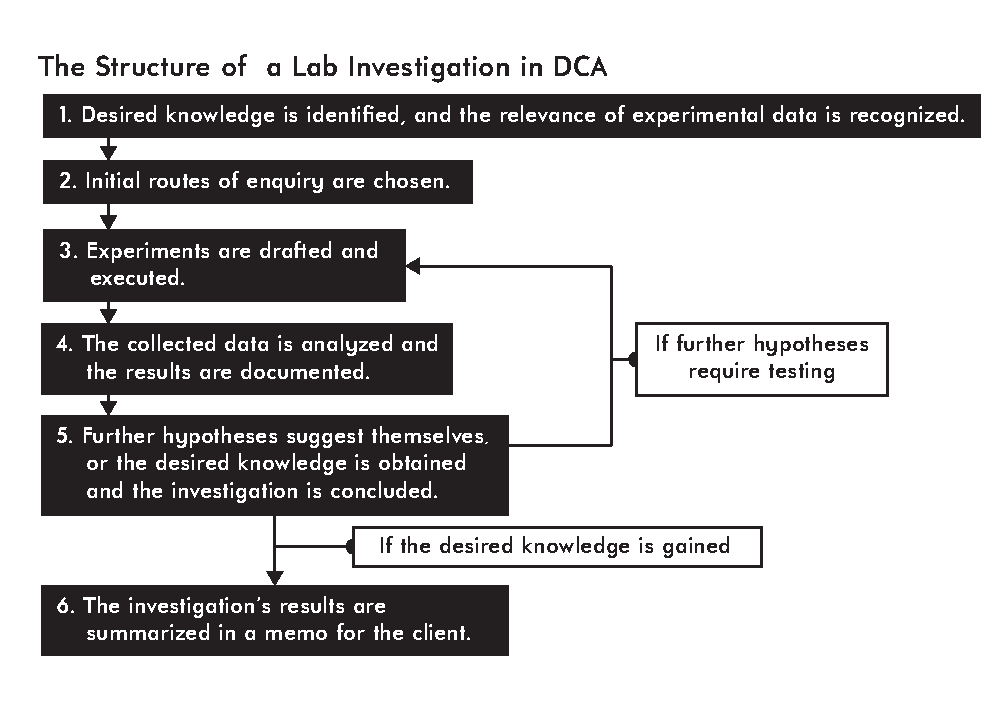
\includegraphics[width=1.2\textwidth]{Lab_Investigation_Diagram.pdf}
\caption{Investigation diagram.}
\label{fig:investigation_diagram}
\end{figure}
% What departments in DCA test their products?
All aspects of an investigation - from experiment design through to presenting the results to a client - are handled by engineers assigned to the project associated with that investigation. Typically investigations focus on a particular product parameter, such as the volume of fluid dispensed by an injector, or the propensity of a inhaler to fail upon being dropped. 
\par
Most lab work is by engineers on medical projects. Occasionally engineers working on fast-moving consumer goods (such as toothbrushes or lotion bottles) will run tests to compare design variations or verify performance relative to some baseline. In general however, the timeframes and functional requirements of such products limit the relevance of extensive experimental investigations to them: medical products on the other hand, see a good deal of the test lab.
\par
% When do they test them and why?
Product testing can be done at any point over a development cycle, however as can be seen in Figure \ref{fig:tests_per_quarter}, the rate of testing increases as a product develops. Towards a product's relase date is when resolving minor performance issues becomes a worthwhile pursuit, exploration for future product variants become a possibility, and rehearsal for fast-approaching regulatory tests becomes essential.
\begin{figure}
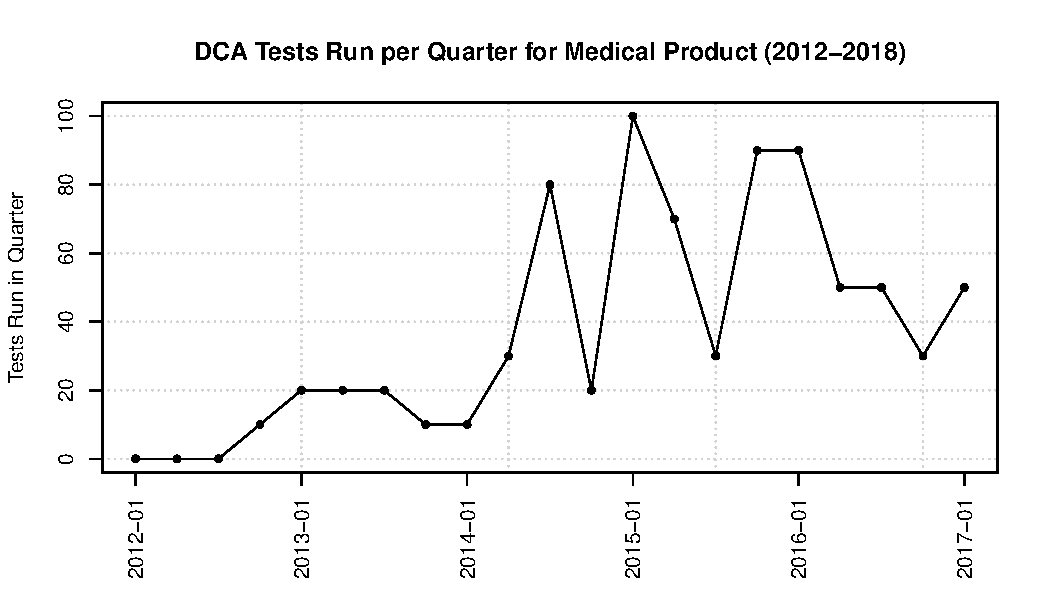
\includegraphics[width=\textwidth]{tests_per_quarter.pdf}
\caption{Frequency of tests in terms of time until project launch.}
\label{fig:tests_per_quarter}
\end{figure}
\par
% How do they test them?
The equipment supporting this work includes axial and torsional testing machines, environment chambers, coordinate measuring machines, mass balances, and high-speed cameras, among other engineering instruments. Investigations commonly revolve around a particular experimental set-up, however other experiments are sometimes conceived to provide supplementary information. With that in mind, this report attempts to be data-agnostic in its recommendations of analytical techniques.
\par
Other engineering activities that DCA's engineers apply statistics to are tolerance analysis and, increasingly, predictive user interfaces. Unfortunately, the latter cannot be discussed for confidentiality reasons; the former can be, and is - see the section on Monte Carlo estimation. Outside of engineering, statistics is used to varying degrees within the Human Factors and upper management od DCA, however these applications aren't talked about here.
\par
To help make sense of how statistics is applied in DCA's lab investigations, its use at each step of an experimental procedure - planning and execution, analysis, and presentation - is discussed in order. For any experimental investigation to be successful, the experiments themselves need to be given careful thought, and should be conducted in a similar spirit. Experiment design aims to guide such thought.

%%
\section{Experiment Design}
Experimental design and analysis can be used to make products that perform better, are more reliable, less risky to develop, and have a uniquely justifiable development process. It is expertise that would elevate DCA's capacity as a technical consultancy.
\par
Design of Experiments refers to both experiment designs and a broader philosophy of systematic experimentation. An experiment design is a particular structure of experiment, such as comparing the effects of two factors each at two levels. Good experimental design produces data that is unambiguous and relevant to an experimental objective.
\par
Three principles are crucial to robust experimentation:
\begin{description}
\item[Replication]{Testing a particular treatment on more than one unit. Replication allows experimental error to be estimated and, since unbiased errors cancel on being averaged, provides a more precise estimate of a treatment's effect.}
\item[Randomization]{Randomly allocating treatments to units and the sequence in which units are tested averages out the effects of nuisance variables, and validifies the important analytical assumption that observations are randomly drawn from a distribution.}
\item[Blocking]{Blocking allows the effects of a nuisance factor to be averaged out during analysis, by accounting for unit differences when assigning treatments - see Figure \ref{fig:blocking}. A block is a set of similar units.}
\end{description}
These constitute the makings of any well-designed experiment, and they are evident in DCA's labwork: units are blocked according to factors such as component batches and time of assembly, testing and assembly sequences are randomized, and engineers are keen to provide replicates in their tests.

\begin{figure}
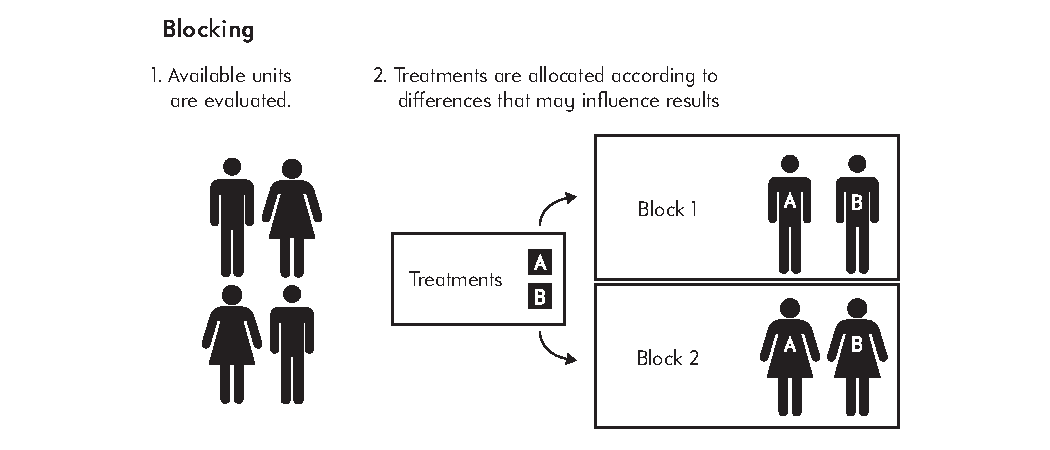
\includegraphics[width=\textwidth]{Blocking.pdf}
\caption{Diagram of what blocking involves.}
\label{fig:blocking}
\end{figure}
\par
This being said, DCA lacks a framework for planning experimental investigations. As a consequence of this, fundamental activities such as verifying that experimental set-ups produce repeatable results, scoping an investigation, and running screening experiments to systematically close off avenues of enquiry are sometimes forgotten. The dominant experimental strategy within the company is a best-guess approach: one treatment is tested in each experiment, chosen based on the expert insight of the engineering team. This method's most serious shortcoming is that if the treatment does not elicit the desired effect, then the next factor to vary must be guessed at, a process that can continue almost indefinitely. Furthermore, if a treatment is successful, then it may be tempting to stop the investigation when a better solution is actually available, allowing luck to play too large a role in a product's design.
\par
DCA's experimental procedure is compared against conventional experimental steps in Table \ref{tab:exp_procedure}.

\begin{landscape}
\vspace*{-3cm}
{\tiny
\begin{longtable}{p{4cm} p{7cm} p{6cm} p{6cm}}
\caption{Comparison of DCA's experimental procedure with conventional practice.}\\
\toprule[0.15em]
\textbf{Experimental step} & \textbf{DCA's implementation} & \textbf{Strengths} & \textbf{Suggestions} \\
\toprule[0.15em]
Recognition and statement of the problem. & A problem is usually identified in either other experiments or design-side activities. It is not formally stated, but is agreed in loose terms among the engineering team. There is no mechanism for assessing whether a problem is well-suited to being addressed by a lab investigation, as opposed to other analytical methods. & The benefits that experimental investigations provide, such as empirical validity and flexibility, are recognized. & A precise problem statement focuses an investigation towards a particular end, and allows progress towards this end to be gauged. It also makes it clear to the team what an investigation aims to achieve. \\ 
 &  &  & Specific problem statements make it easier to review previous work - without them, it is difficult to determine where one investigation begins and another ends. \\ 
\cmidrule{1-4}
Choice of factors, levels, and ranges. & This choice is made in engineering team meetings. Factors can be identified haphazardly: there is no labelling of those that are identified as design or nuisance factors, or whether they are controlled or uncontrolled. Ranges and levels are usually chosen according to expert knowledge. The number of levels is usually kept small (2 or 3) because differences rather than overall responses are of interest. & Level choices have a rational motivation which is justified via physical reasoning or previous experimental results. & A list of factors guides the systematic elimination of sources of variation from an experimental set-up, and can be used to survey for possible confounding factors. \\ 
 &  & Deciding which factors are relevant in a meeting uses the entire team's engineering knowledge and critical thinking skills. & A meeting should be a place to review a choice, not to generate it - conversation is not methodical and can easily miss relevant information. \\ 
\cmidrule{1-4}
Selection of the response variable. & The response variable is usually evident from the problem statement (e.g. torque output of mechanism). More than one way to measure the response variable will almost always be considered. & Engineers in the company can generate many possible response variables, and analyze their respective merits. & Precursor experiments comparing response variables may reduce the length of investigations. \\ 
 &  & The response variable chosen is chosen carefully to closely represent the system under study. & Documenting the alternative response variables would make it easier to clearly outline why one method is superior, and to transition between testing methods as circumstances change. \\ 
\cmidrule{1-4}
Choice of experimental design. & The experimental design is also chosen in a meeting. They are usually one from a small selection (detailed in the text body). The choice made is incidental, as reflected by the absence of planning documents. & Simple experiment designs are easily communicated, executed, and documented. & A well-chosen experimental design can reduce the resources (time, materials, and effort) expended in satisfying the investigation's objective. \\ 
 &  &  & Considering analysis beforehand makes it possible to ensure analytical assumptions are met. \\ 
\cmidrule{1-4}
Performing the experiment. & Engineers run their experiments in a laboratory. Frequently run experiments have protocols; hand-written observations are mandated for all experiments. & Labs afford flexibility in the level of experimental control. & Experimental fixtures should be shown to generate repeatable, reliable results before being used. \\ 
 &  & Blank observation sheets encourage critical thinking about the experiment & Images of test set-up would make it much easier to retrospectively understand an experiment. \\ 
 &  & Experiments are run by engineers solving the problem - this makes engineers personally responsible for their results, and exposes them to undocumented experimental information. & Observation sheets could provide guidance on what factors to monitor. \\ 
\cline{1-4}
Analysis of the data collected. & Analyses are run as soon as data is available, and will be handled by the engineer that ran the experiment. Excel - and occasionally Matlab - is used. The conclusions tend to be judgemental as opposed to statistical. Compared to the time spent running the experiment, analysis is brief. Analysis is discussed in more detail in the next section. & Engineering expertise is applied to explain experimental results in a physically meaningful way. & Statistics should be used to ensure that sound conclusions are made - subjective assessment alone is susceptible to various biases that can lead to lost time and confusion. \\ 
 &  &  & Time invested in analyses should be seen as what makes an experiment practically useful, rather than a formality between experiments. \\ 
\cmidrule{1-4}
Conclusions and recommendations & Conclusions are incorporated into client memos and presentations. Interim results are presented at internal meetings - graphics play an important role in communicating results. & The importance of graphics is realized and put to good effect in client presentations. & Charts exist beyond those being used that may make it easier to demonstrate experimental results. \\ 
 &  & Conclusions are presented in a way that is accessible and avoids needless technicalities. & Experimental results are not supplemented by estimates of uncertainty. \\
\bottomrule
\label{tab:exp_procedure}
\end{longtable}
}
\end{landscape}


\par
The experimental designs used in the company are enumerated, explained, and critiqued in Table \ref{tab:exp_designs}. As mentioned, the core problem with DCA's experimental strategy is its narrow focus on testing specifics - running a few large experiments considering many different treatments at once can be much more efficient than many very specific experiments. Moreover, there is no understanding of what constitutes a statistically efficient design -...
\renewcommand\arraystretch{1.5}
\begin{table}[H]
\hspace*{-2.25cm}
\small
\centering
	\begin{tabular}{p{3.5cm} p{6cm} p{6.5cm}}
	\toprule
	\textbf{Experimental Design} 		& 	\textbf{Description}	&	\textbf{Evaluation} \\\toprule
	Randomized complete block design	 & 	Each treatment is randomly assigned to at least one unit from every block. &  Allows the effects of nuisance variables to be eliminated during analysis, provided the block factor and treatment do not interact. \\
	& & Lends itself to established analytical techniques (e.g. ANOVA). \\
	& & Can be extended to block on more than one factor (such a design is called a Latin square) \\
	& & Not possible if the number of units in a block is fewer than the number of treatments to be tested. \\
	&&\\
	Factorial design & Applied to experiments in which more than one factor is varied - all combinations of factor levels are tested. & More time-efficient than testing one factor per experiment. \\
	& &  May be limited by resources if there are many factors \\
	& & Allows interaction effects to be estimated.
	\\\bottomrule
	\end{tabular}
	\hspace*{-2.25cm}
	\caption{Experimental designs applied in DCA.}
	\label{tab:exp_designs}
\end{table}

After an experiment is designed, it must be run. DCA is very well endowed to run experiments, and has a system in place for documenting the date, purpose, and conditions of an individual experiment. Systematically identifying and stating whether factors are controlled would allow the company to make more effective use of its experimental equipment - things are easily forgotten, and mishaps can easily be avoided through a little forethought. 

Once an experiment has been planned and run, it remains to analyze the raw data to extract useful information. A well-designed experiment's analysis should write itself - the purpose should be evident from the beginning. Methods for constructing an analysis are now discussed.

\newpage
%%
\section{Analysis of Experimental Data}
The content of several hundred test reports was tabulated to inform this discussion, which focuses on summary statistics and interval estimates.
\par
Analyses in DCA rely heavily on expert knowledge of the systems being tested and rarely on statistical results. This is probably because the relevance of statistics may not be clear, and how it might be applied even less so, which is understandable. It's widely agreed that most people's experience with statistics is one of discomfort and bemusement. Having said this, relying on intuition alone risks falling prey to cognitive biases, missing valuable information that isn't superficially obvious, and being unable to properly relate physical behaviours to experimental observations. Foregoing statistics when analyzing product behaviour severely handicaps the ability of an engineer to design a robust product.
\par
The reports surveyed contained summary statistics, such as arithmetic means, variances, maximums, minimums, and so on. A few made use of interval estimates as informed by a regulatory standard, and one report applied a t-test. These tools will now be explained, and their usefulness and possible weaknesses detailed.
\par
\subsection*{Summary Statistics}
 Randomness simply means variation in an event as a result of unseen factors. A random variable (r.v.) is a function that maps events onto real numbers. For example, we could define an r.v. $X$ that maps the outcomes of a coin toss onto the numbers 1 and 0:
 \begin{align}
	X(\texttt{Coin lands Heads}) = 1 \\
	X(\texttt{Coin lands Tails}) =0
 \end{align}
Usually the choice of mapping is quite natural - for example, we might use an r.v. that counts the number of sucesses in many trials, or that takes on the value of a measurement. 
\par
Variation in the events that an r.v. maps from is described using a probability distribution. Each value is weighted according to its probability or, in the case of continuous-valued r.v.s, the ratio of the width of an interval of values to its probability. Figure \ref{fig:example_pd} highlights this difference.
\par
The essential problem of experimental statistics is trying to understand the behaviour of a broader population from just a sample. In product design, this means estimating the distribution of a population using measurements from just a limited number of prototypes. The attributes of this distribution - such as its spread and average - can be estimated using summary statistics.
 \par
A sample's mean response, for example, approximates the mean response of a population. This result is regularly used in DCA to discriminate between the performance of two or more populations, each representing possible design variants. The accuracy of this estimate improves as more samples are tested, with diminishing returns, a relationship that is shown in Figure \ref{fig:se_with_sample_size}. Because a sample may not be representative of its population, it's usually useful to understand how far off the sample mean could be from the true mean.The sample mean's average difference to the true mean is called the standard error, and it corresponds to $\frac{\sigma}{\sqrt{n}}$, where $\sigma$ is the standard deviation of the population and $n$ is number of units in the sample. DCA implicitly appeal to this relationship when they choose to run more units in a test, recognising that bigger samples tend to better represent their populations.
\begin{figure}[h]
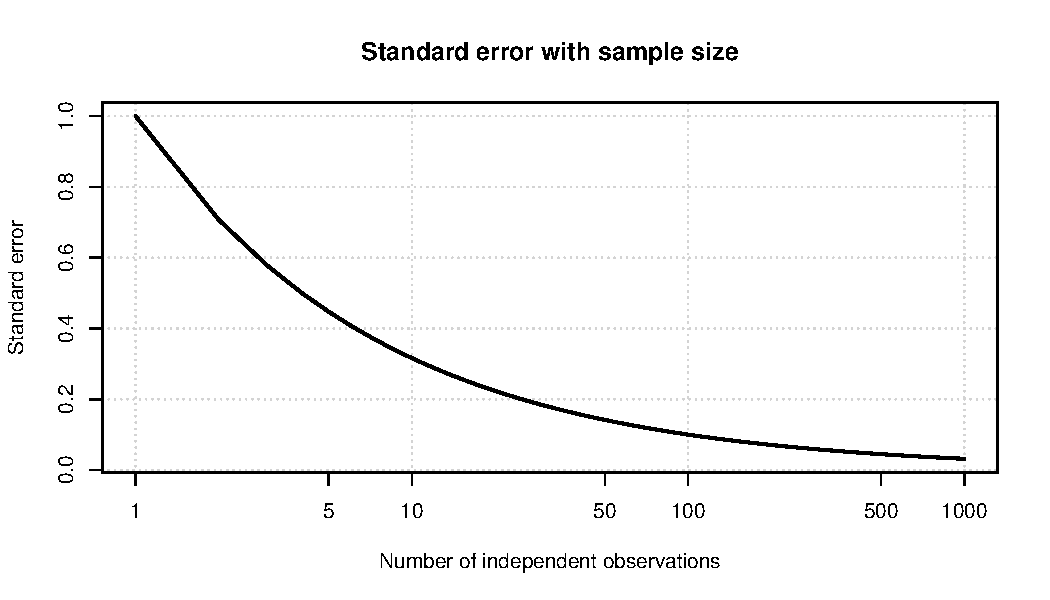
\includegraphics[width=\textwidth]{se_with_sample_size.pdf}
\caption{Convergence of sample mean to population mean.}
\label{fig:se_with_sample_size}
\end{figure}

Certain summary statistics can be thought of as estimates of a distribution's parameters. These are values that constrain a particular distribution's shape. The normal distribution's shape, for example, can be specified by supplying just two values: the variance (spread) and mean (location). Viewing statistics as an exercise in estimating a distribution makes handling the uncertainty inherent in test results more natural, and avoids misleading people with small-sample point estimates. DCA's engineers at particularly at risk of the latter because their experiments are usually constrained by the number of units that can be tested.

 Estimating a distribution will be seen again later, in the section on Bayesian inference. Interval estimates are a tool for quantifying the uncertainty on an estimate, and can be made with assumptions about the distribution's shape, or without. They need to be interpreted carefully, and an appropriately careful explanation of two of the most often used interval estimates - confidence and tolerance intervals - will now be presented.

\begin{figure}
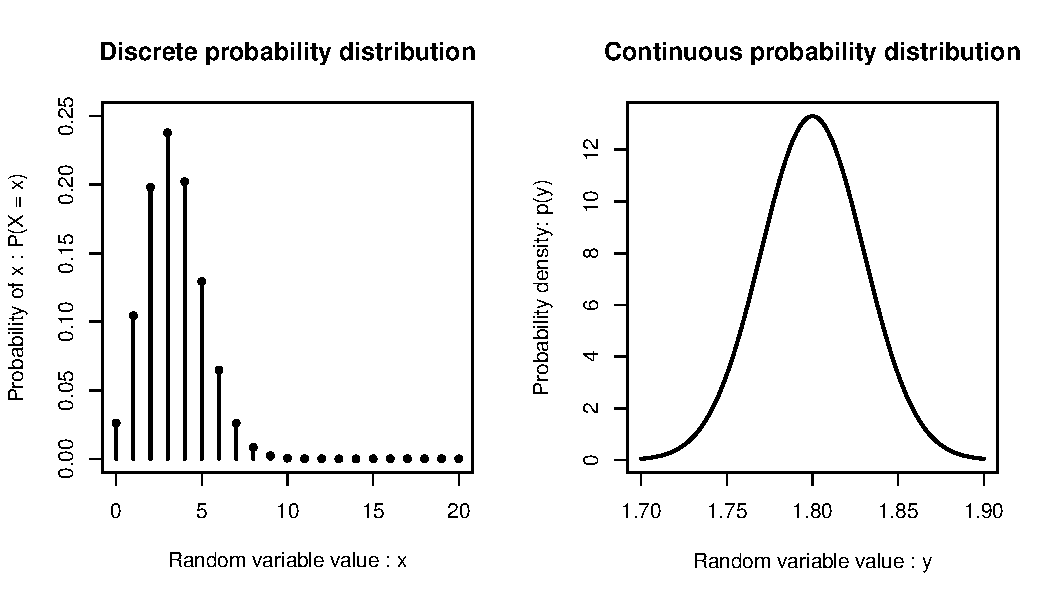
\includegraphics[width=\textwidth]{probability_distributions.pdf}
\caption{Left: Probability mass function. Right: Probability density function.}
\label{fig:example_pd}
\end{figure}
\par

\newpage
\subsection*{Tolerance Intervals}
DCA's most sophisticated statistical analysis is based on ISO 16269-6, \emph{Determination of statistical tolerance intervals}. This standard outlines how to construct tolerance intervals under either no assumptions about the random variable's distribution, or the assumption that the random variable has a normal distribution. A tolerance interval is a range of values that contain a particular fraction of the population. Because this interval is only an estimate, they can only contain the advertised fraction of the population most of the time. The proportion of time that an interval would, on average, contain the specified fraction of the population is called the confidence level. To elaborate a little further, if many $99\%$ tolerance intervals were constructed for different samples of the same size to a $95\%$ confidence level, then $95\%$ of the intervals estimated would contain at least $99\%$ of the population. Figure \ref{fig:tolerance_intervals} shows what this means.

So tolerance intervals allow us to make statements about the performance of a population, with clear limits on that statement's uncertainty. Tolerance intervals are derived by thinking about the probability that a member of the population will be within a particular range. For a one-sided tolerance limit - a value for which at least $p\%$ of the population is greater than or less than - this means:
\begin{enumerate}
	\item Defining $k$ such that the probability a member of the population $(mu + u sigma)$ is greater than $k$ sample standard deviations from the sample mean is eqaul to $1 - a$.
		\begin{equation}
			P(\bar{x} + ks \geq \mu + u_p \sigma) = 1 - \alpha
			\label{eq:tol_interval}
		\end{equation}
	Where $\bar{x}$ is the sample mean, $s$ is the sample standard deviation, $\mu$ is the true mean of the population, $\sigma$ is its true standard deviation, and $u_p$ is such that $\mu + u_p\sigma$ is greater than $p\%$ of the population. $\alpha$ is the confidence level. \newline In words, $k$ is such that $\bar{x} + ks$ will  be greater than the $p\%$ of the population $(1 - \alpha)\%$ of the time.
	\item Assuming $x$ has a normal distribution then $u_p$ can be read off a table of normal values, and by definition $\frac{(n-1)s^2}{\sigma^2}$ will have a chi-square distribution (see Appendix A). What this means is that $k$ has the same distribution as a $t$-distributed r.v. centered at $\sqrt{n}u_p$ and scaled by $\frac{1}{\sqrt{n}}$:
		\begin{equation}
			k = \frac{1}{\sqrt{n}}t_{n - 1}(\sqrt{n}u_p) 
		\end{equation}
		This is a normal distribution that's more spread out - the bigger spread represents the uncertainty on account of the fact that the true variance isn't known.
	\item  Bonanza! The lower interval containing at least $95\%$  of the population is
\begin{equation}
	\Big(-\infty, \bar{x} + \frac{t_{1 - \alpha}(\sqrt{n}u_p, n - 1)\cdot s}{\sqrt{n}}\Big]
\end{equation}
A fraction $1 - \alpha$ of these intervals will contain less than $p\%$ of the population, as shown in Figure \ref{fig:tolerance_intervals}. 
\end{enumerate}
DCA use tolerance intervals in a particular test to check that a certain proportion of the population satisfies a performance threshold. Their use isn't widespread, and previously it's been the case that $k$ values haven't been properly updated according to the conditions of new tests.


\begin{figure}[H]
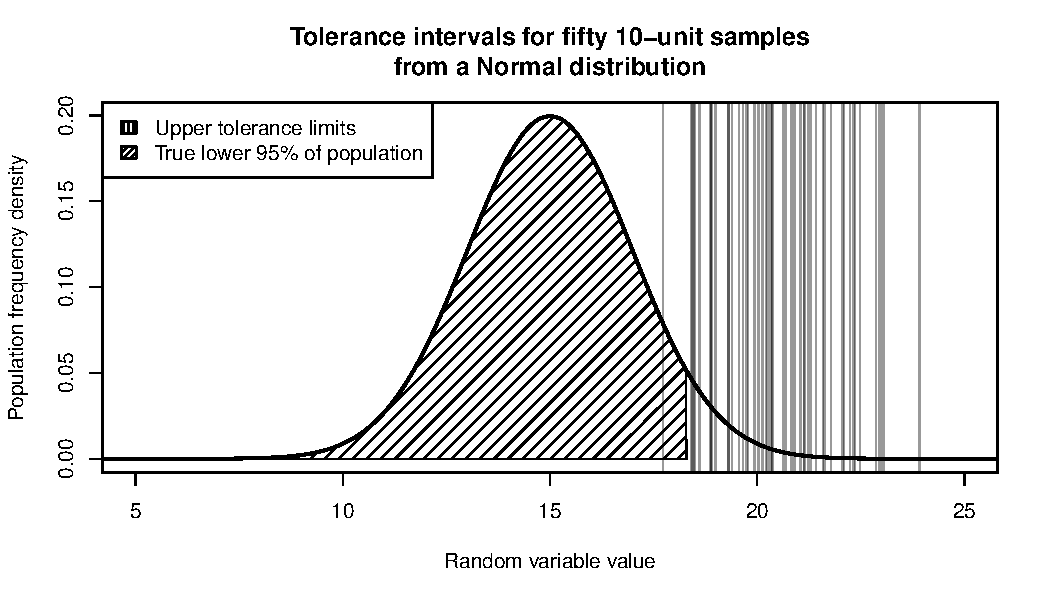
\includegraphics[width=\textwidth]{tolerance_intervals.pdf}
\caption{Twenty tolerance limits versus population limit.}
\label{fig:tolerance_intervals}
\end{figure}
The strengths and suggestions for DCA's tolerance intervals are listed in Table \ref{tab:tol_intervals}.
\begin{table}[b]
\caption{Evaluation of tolerance intervals.}
\small
\hspace*{-.5cm}
\begin{tabular}{p{6.5cm}p{6.5cm}}
\toprule
\textbf{Strengths}	&	\textbf{Shortcomings} \\
\toprule
Provides a threshold indicating roughly where a certain fraction of the population is. & Confidence levels can be misinterpreted as specifying the probability that a constructed interval contains at least $95\%$ of the population. \\
In line with the expectations of regulatory standards & Normality assumption needs checking \\
Can be setup to be applied without theoretical understanding & Repeated use at a low confidence level increases the probability that the limit will be under-estimated. \\
& k-values need to be looked up - could easily be done incorrectly if the theory isn't understood.\\
\bottomrule
\end{tabular}
\label{tab:tol_intervals}
\end{table}

\newpage
% Confidence intervals
\subsection*{Confidence Intervals}
Another tool that DCA's engineers occasionally use is confidence intervals, which indicate a range of values that a parameter is likely to fall within. As with tolerance intervals, this range will only contain the population parameter a certain fraction of the time however, a problem that's unavoidable since there will always be a chance that an unrepresentative sample is drawn. For example, if we were to construct a confidence interval for the population mean of 100 samples, each of 5 units, the confidence level would tell us how many of these intervals would - on average - contain the actual value of the population mean. Figure \ref{fig:confidence_intervals} demonstrates this idea. Confidence intervals can be placed on any parameter estimate, although they're usually used to quantify the uncertainty on an estimate of the population mean. Their derivation is similar to a tolerance interval's:
\begin{align}
	\text{P}(\bar{x} - ks \leq \mu \leq \bar{x} + ks) &= 1 - 2\cdot \text{P}(\bar{x} - ks \leq \mu) = 1 - \alpha \nonumber\\
	\implies \frac{\alpha}{2} &= \text{P}(\frac{\bar{x} - \mu}{s} \leq k) 
\end{align}
The last line implies that $k$ has a $t$-distribution with $n - 1$ degrees of freedom, so that the confidence limit that contains the true mean $(1 - \alpha)\%$ of the time is
\begin{equation}
	[\bar{x} - t_{n-1}(\alpha)\cdot s, \ \bar{x} + t_{n-1}(\alpha)\cdot s]
\end{equation}
\begin{figure}[H]
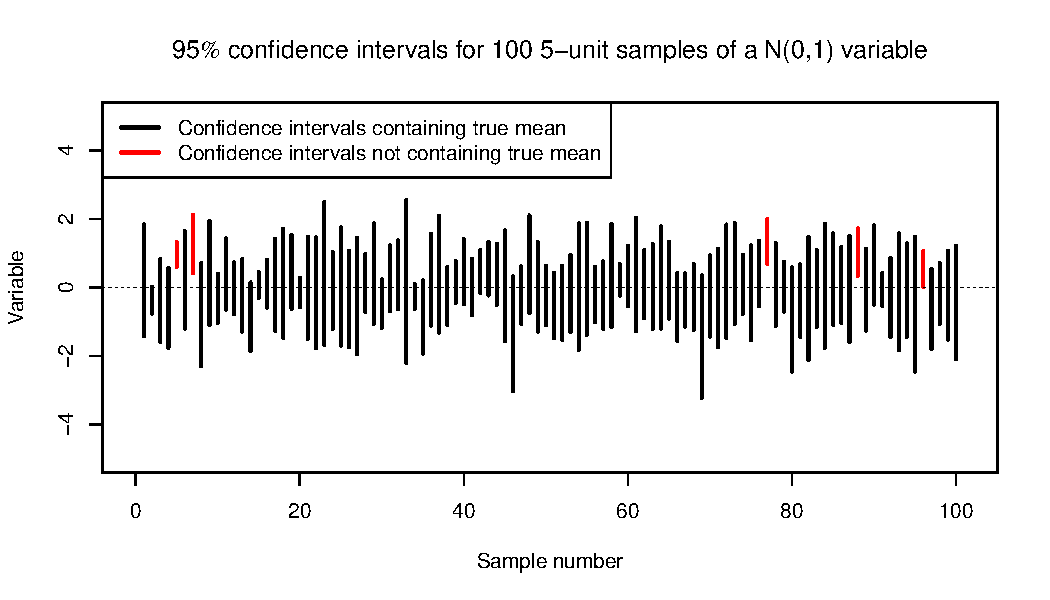
\includegraphics[width=\textwidth]{confidence_intervals.pdf}
\caption{99$\%$ confidence intervals, to a $5\%$ confidence level, for 100 10-unit samples.}
\label{fig:confidence_intervals}
\end{figure}
Confidence intervals suffer from similar problems to tolerance intervals. DCA's engineers use them very rarely.

\newpage
\subsection*{Monte Carlo Estimation}
Monte Carlo estimation approximates a quantity by simulating the random process generating it . In DCA it's been used to analze tolerance chains in products. The use case was somewhat similar to the following: the tolerance limit of a combination of distributions, each corresponding to a part dimension, was needed. Take $X \sim \text{Binom}(n = 10, p = Y)$ as an example, where $Y \sim \text{Beta}(a = 7, b = 3)$\footnote{The beta distribution is a continuous and generates a number between $0$ and $1$, which makes it useful in modelling the distribution of a probability.}. Rather than attempt to derive the distribution of this dimension's value directly, tens of thousands of values of $y$ were first generated according to $Y$'s distribution using a computer. Each of these values were then used to generate a value of $x$ from $\text{Binom}(n = 10, p = y)$. The resulting frequencies of the $x$ values then represented the dimension's distribution. It was then possible to calculate the mean by averaging over all the $x$ values obtained. A diagram of this process is shown in Figure \ref{fig:monte_carlo}.
\begin{figure}[b!]
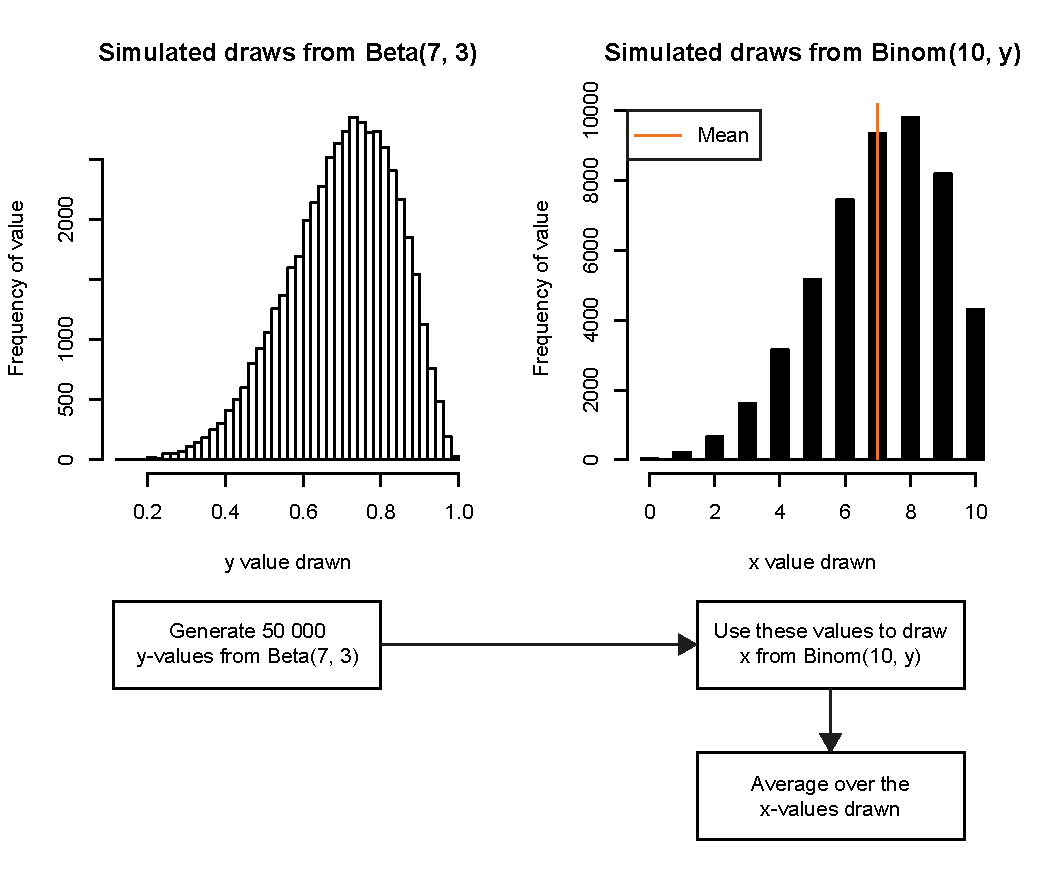
\includegraphics[width=0.87\textwidth]{monte_carlo_simulation.pdf}
\caption{Process diagram for a Monte Carlo simulation.}
\label{fig:monte_carlo}
\end{figure}


\newpage
\section{Visualizing Experimental Data}
Visualization is essential to clearly and convincingly summarizing an experiment's results. Graphical tools allow engineers and clients to see for themselves what's been discovered. A plot should relevant, easily interpretable, and accurately convey its underlying data.
\par
DCA's reports and client presentations frequently contain plots of the data collected from an experiment, typically generated using either Microsoft Excel or Matlab. The plots used are line and bar charts, along with the occasional scatterplot. Line charts are particularly ubiquitous in DCA because they're directly plottable from the raw data provided by axial and torsional testing machines. As a consequence of this many graphical summaries are usually overlaid line plots, similar to that shown in Figure \ref{fig:line_chart}. The effectiveness of this use-case is evaluated in Table \ref{tab:line_chart}. This type of plot can include a lot of redundant information and can make it difficult to see how individual units are behaving.  Line charts can also conceal the actual resolution of the data collected, particularly if a spline fit or graphical smoothing has been applied\footnote{As is a default in Excel.}. Figure \ref{fig:line_chart} is a representative chart from a DCA test report showing an overlay of the results from many units. Criticisms aside, directly plotting raw data requires very little time, and is easily relatable to patterns observed over the course of an experimental run.
\begin{figure}
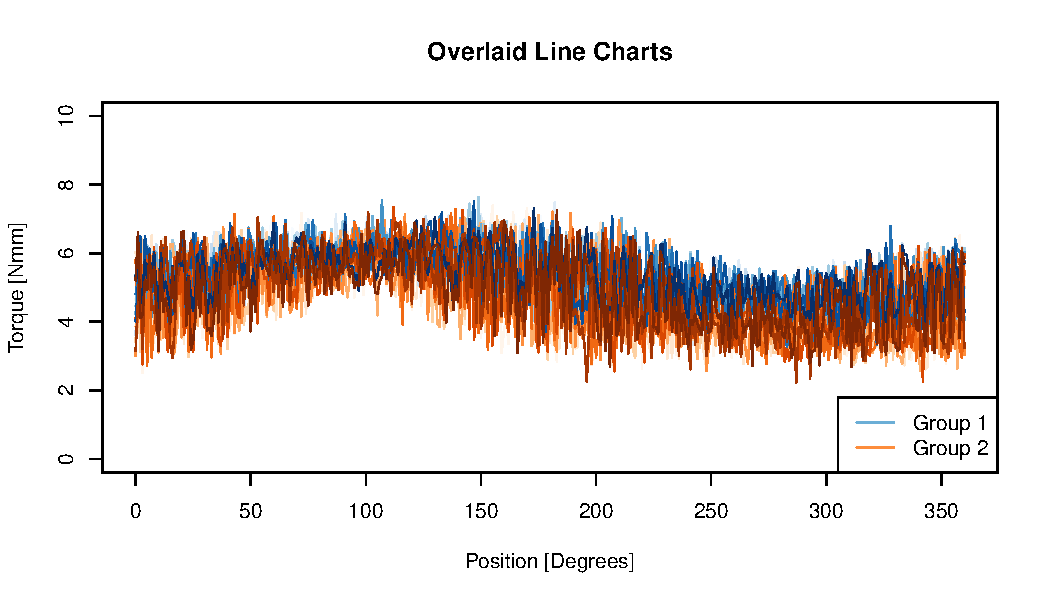
\includegraphics[width=\textwidth]{overlaid_line_charts.pdf}
\caption{A representative use of line charts from a DCA test report.}
\label{fig:line_chart}
\end{figure}

Bar charts are also used fairly frequently to display performance relative to a nominal value, and a particular format of scatterplot is used to present the results of a tolerance limit analysis. The latter is shown in Figure \ref{fig:tolerance_intervals_plot}. 
\begin{table}[h!]
\caption{Evaluation of the line chart.}
\small
\hspace*{-.5cm}
\begin{tabular}{p{6.5cm}p{6.5cm}}
\toprule
\textbf{Strengths}	&	\textbf{Shortcomings} \\
\toprule
Allows an entire test to be viewed simultaneously, providing a high-level summary of results.	&	May provide irrelevant information - it's often the case that only the peak or average values are of interest	\\
Is easily relatable to physical observations during a test.	&	Directs focus to extremes of group ranges, rather than the distribution of each group's performance.	\\
Its meaning can be understood without explanation - it is a universally familiar chart.	&  Obfuscates data artifacts that aren't related to location or dispersion (such as harmonic content). \\
&  Can obscure the behaviour of individual units. 			\\
\bottomrule
\end{tabular}
\label{tab:line_chart}
\end{table}
\begin{figure}
	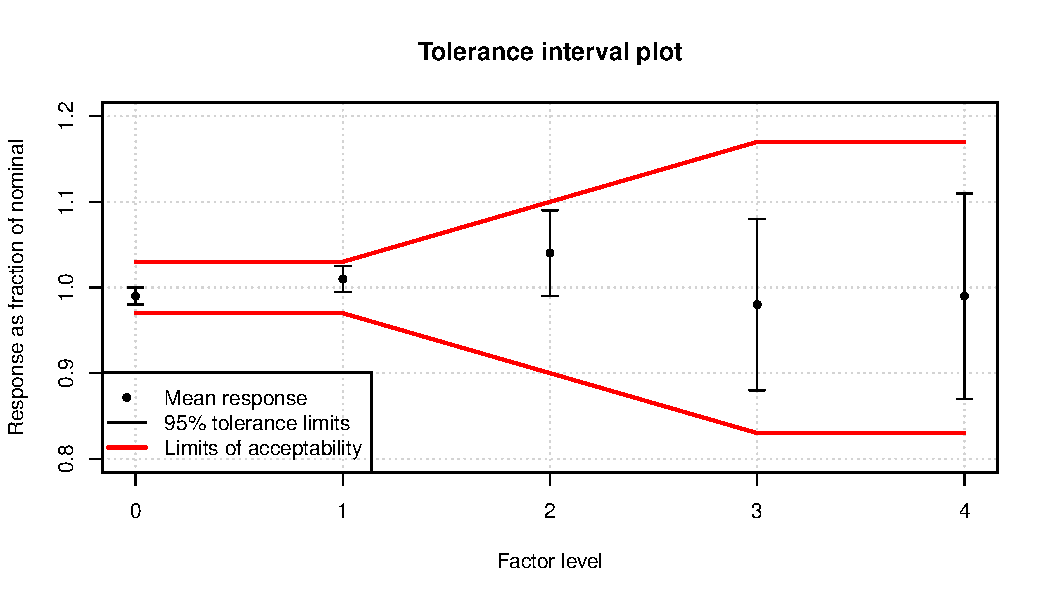
\includegraphics[width=\textwidth]{tolerance_intervals_plot.pdf}
	\caption{Tolerance interval plot.}
	\label{fig:tolerance_intervals_plot}
\end{figure}

\section{Review}
The report so far has presented and critiqued the statistical methods currently being used by DCA's engineers. ...CONTINUE


\newpage
%%  SUGGESTED METHODS %%
\chapter{Suggested Methods}\label{suggested_methods}
\label{chap:modernstats}

Having assessed DCA currently uses statistics, it's possible to suggest methods from modern statistical practice that would give them new capabilties and improve their existing attempts. This section again is structured according to the steps in an experimental process.

\section{Experiment Design}
Experiments design is motivated by trying to find efficient ways to explain variation in performance. To understand what factors determine a product's performance, this variation must be split into components attributable to product factors. The factors can be tuned to produce a desirable response. Experimental investigations should be planned to methodically work out what the effects of factors are on the response, with the available resources. Response surface methodologies would allow DCA's engineers to do this in a way that is resource-efficient, and is in some measure plannable.

\subsection*{Response Surface Methodologies}
In any given one of DCA's products, it's likely that most parameters will either need to be:
\begin{itemize}
	\item Kept within a range - for example, criticial dimensions
	\item Maximized or minimized - such as mechanism friction or split line prominence
\end{itemize}
Response surface methodologies try to achieve these objectives by sequentially identifying the factors that affect the response parameter. The general idea is to:
\begin{enumerate}
\item Start by determining what the first-order effects of factors are on the response. In other words, estimate the coefficients in the model:
\begin{equation}
	f(x_1, ..., x_n) = x_0 + \sum_{i = 1}^n \beta_i \cdot x_i
\end{equation}
\item Incrementally optimize the response based on the model. If the response were being maximized, this would mean adjusting the factors $x_i$ until the reponse $f(x)$ stops increasing. 
\item Determine what the second-order interaction effects are in the vicinity of the first-order optimum. That is, fit a model of the form:
\begin{equation}
	f(x_1, ..., x_n) = x_0 + \sum_{i = 1}^n \sum_{j = 1}^n \beta_{ij}\cdot x_i \cdot x_j
\end{equation}
\item Optimize the response according to these second-order effects (described in the Appendix).
\end{enumerate}
Something missing from the above steps is that a shot of common sense is needed at each stage - factors that have a negligible effect on the response need to be discarded to avoid having to test a staggering number of second-order treatments to test. The structure of an RSM assumes that first-order effects are likely to be larger than interactions. 

To estimate first-order effects, two factor levels need to be defined, then every combination of factor levels - $2^k$ in total - need to be tested.  To estimate error of course, replicates of each combination of factors need to be tested. To make these estimates more efficient, replicates at only a few points can be run. If these points are centered relative to the other factors, then they can suggest whether the changes seen moving towards the surrounding points are probably attributable to error or an effect. Figure \ref{fig:centered_points} shows what a center point is.

Central composite designs can be used to fit the second-order model: these consists of a testing all combinations of factors, replicating at the center points described above, then displacing one factor at a time from each of these center points. This type of experiment provides just the right amount of information to characterise the reponse surface around the center points (see the Appendix's discussion of orthogonality).

\begin{figure}
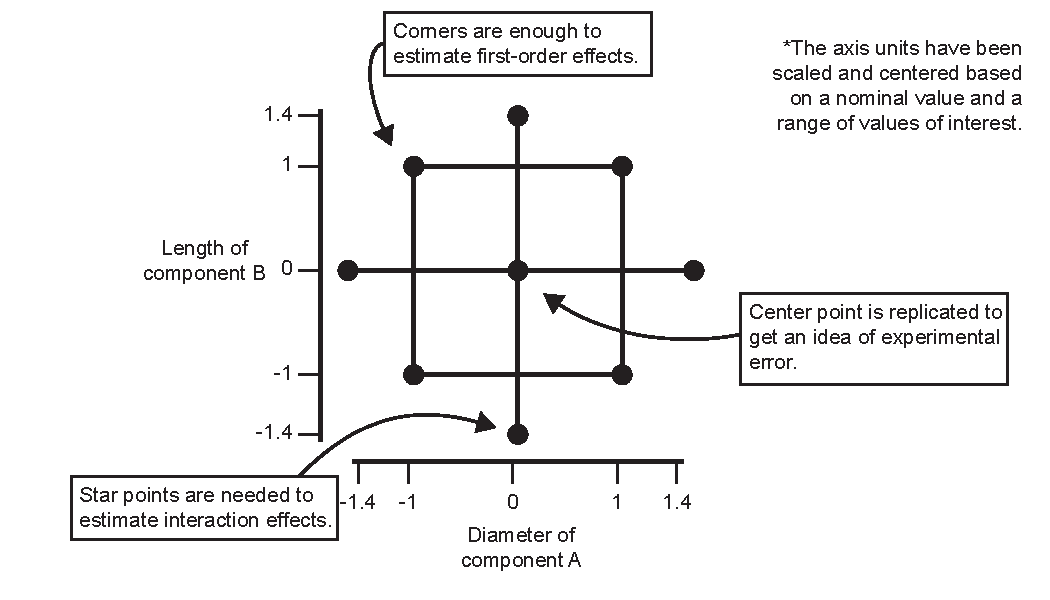
\includegraphics[width=\textwidth]{central_composite_design.pdf}
\label{fig:centered_points}
\caption{A central composite design - the points indicate factor combinations to be tested, and the lines suggest the experiment's intentions.}
\end{figure}

 DCA could use response surface methodologies to converge more quickly on a solution than their current best-guess approach. Additionally, the solutions found using this method would be approximately optimal, rather than sufficient - this means better products, and more satisfied clients. It can be difficult to get hold of the resources to run a large experiment, and to convince a client that it will be worthwhile, but perserverance will repay itself in the risk, possible embarassment, and possible loss of business avoided as a result. Furthermore, investigations relying on - admittedly expert - guessing will consume more resources than planned investigations. The experiment designs presented here provide an idea of the minimum up-front cost needed to understand the effects of a set of factors on a response. If this cost is too high, and the factors can't be reasonably discounted, then the objectives of the investigation should be refined.


\newpage
\section{Analysis}
\subsection*{Regression Analysis}
% What's a regression model?
% How's it useful to DCA?
% What do they consist of?
% What are their limitations, and how can they be applied to more difficult problems?
Experimental work often tries to an answer questions such as:
\vspace{-10pt}
\begin{itemize}
\item Which factors are having a big effect on the response?
\item How does a factor affect the reponse? How do several factors interact?
\item Which design variation is better?
\end{itemize}
\vspace{-10pt}
 Regression analysis would allow DCA's engineers to answer questions like these. Knowing what parameters affect the product, and by how much,  focuses development on the things that matter, resulting in a better quality product that's less risky to develop.
 \par
 Regression estimates how a continuous response changes with some inputs. Linear regression uses a linear function to predict the reponse: This may sound limiting, since in real life lots of relationships are nonlinear, but nonlinear relationships can be made linear by transformation.
\par
  Linear models describe a response $y$ as a linear function of some parameters $\hat{\beta}_i$, each weighted by a corresponding input $x_i$. An example of such a model would be:
\begin{equation}
	\hat{y} = f(x_1, x_2) = \hat{\beta}_0 + \hat{\beta}_1 \cdot x_1 + \hat{\beta}_2 \cdot e^{x_1}+ \hat{\beta}_3 \cdot x_1 \cdot x_2
\end{equation}
Where $\hat{y}$ is the estimated response, $x_i$ is an input, and $\hat{\beta}_j$ is the coefficient of the $j$th input. Note that while the coefficients $\hat{\beta}_j$ are linear, the predictors $x_j$ can be nonlinear functions of the measurements.

This model can be fit by adjusting the $\hat{\beta}_i$ values so that $\hat{y}$ is a good estimate of the true response. To do this, it's necessary to measure how inaccurate $\hat{y}$ is relative to $y_i$. One way of measuring fit inaccuracy is the residual sum of squares:
\begin{equation}
	\text{RSS}(\hat{\beta}) = \sum_{i = 1}^m \Big(y_i - \sum_{j = 1}^p \hat{\beta}_i x_{ij})^2
	\label{eq:rss}
\end{equation}
Where $y_i$ is the response of the $i$th example, and $x_{ij}$ is the $j$th predictor value of the $i$th example. This measure of fit is a good one for several reasons, the most intuitive of which is that it minimizes the overall distance between the estimates $\sum_{j = 1}^p \hat{\beta}_j x_{ij}$ and the responses $y_i$ \footnote{The residual refers to the difference between an estimated response and a true response at a particular set of inputs. Error refers specficially to deviation of a response around its expected value.} . There are two alternative justifications for least squares, which are both presented in the Appendix.

 Figure \ref{fig:linear_regression}. 
\begin{figure}
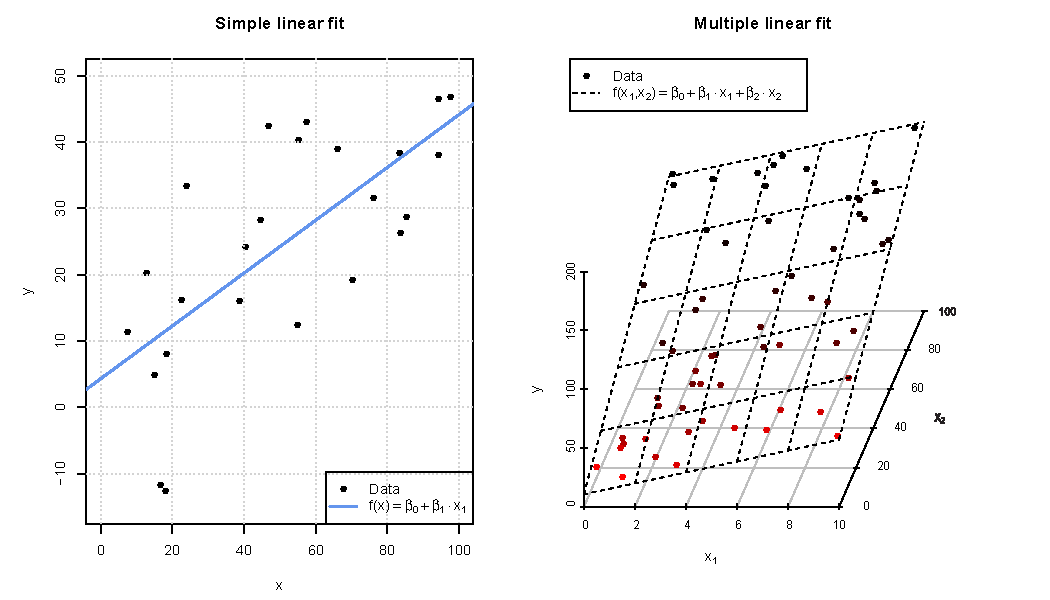
\includegraphics[width=\textwidth]{linear_fits.pdf}
\caption{A simple and a multiple linear fit.}
\label{fig:linear_regression}
\end{figure}

From a practical standpoint, regression models should be fit using software. Matlab, R, or Octave can all be used to fit regression models. By setting up the problem such that the $N$ observed responses are in a column vector $\mathbf{y}$, their associated $p$ inputs form the rows of a matrix $\mathbf{X}$, which is $N \times p$, and the $p$ coefficients are in a column vector $\hat{\beta}$, it's possible to succinctly write the RSS criterion, then minimize it:
\begin{align}
	\text{RSS}(\hat{\beta}) &= (\mathbf{y - X}\hat{\beta})^T(\mathbf{y - X}\hat{\beta}) \\
	\frac{\partial \text{RSS}}{\partial \hat{\beta}} &= -2\mathbf{X}^T(\mathbf{y - X}\hat{\beta}) = 0 \\
	\implies &\hat{\beta} = (\mathbf{X}^T\mathbf{X})^{-1}\mathbf{X}^T \mathbf{y} \label{eq:normal_eqtn}
\end{align}

As a case study to show why linear models are useful, consider a test in which the load delivered by three groups of ten units is measured. The differences between the groups are categorical: the groups correspond to three design variations $A, B,$ and $C$. Since there isn't a natural order to the variations, it's necessary to encode this difference in a sensible way. There are several ways to do this, and a simple indicator stating whether a unit has a particular modification is sufficient. Table 5 shows this encoding. As will hopefully become apparent, choosing how to encode categorical variables matters a good deal with regards to how the regression coefficients beta should be interpreted.
\begin{table}
\centering
\caption{Dummy coding of groups.}
\small
\begin{tabular}{c c c c c}
\toprule
\textbf{Unit ID}                 & $\mathbf{x_A}$ & $\mathbf{x_B}$ & $\mathbf{x_C}$ & \textbf{Load, $\mathbf{y}$ [N]} \\
\midrule
1                       & 1 & 0 & 0 & 5.43         \\
2                       & 0 & 1 & 0 & 7.48         \\ 
& & \vdots & & \\
30 & 0 & 1 & 0 & 6.47 \\
\bottomrule
\end{tabular}
\end{table}

Next the model is set up:
\begin{gather}
	\hat{y} = \hat{\beta}_0 x_A + \hat{\beta}_{1}x_B + \hat{\beta}_{2}x_C = x \hat{\beta} \label{eq:categorical_regression} \\[5mm]
	\mathbf{X} = 
		{\tiny
			\begin{bmatrix}
				x_1 \\ x_2 \\ \vdots \\ x_{30}
			\end{bmatrix}
			=
			\begin{bmatrix}
				 1 & 0 & 0 \\  0 & 1 & 0 \\ \vdots & \vdots & \vdots \\ 0 & 1 & 0
			\end{bmatrix}}
	\quad \mathbf{y} = {\tiny \begin{bmatrix} 5.43 \\ 7.48 \\ \vdots \\ 6.47 \end{bmatrix}}
	\quad \hat{\beta} = {\tiny \begin{bmatrix} \hat{\beta}_0 \\ \hat{\beta}_1 \\ \hat{\beta}_2 \end{bmatrix}}
\end{gather}
We can then use the normal equation (Equation \ref{eq:normal_eqtn}) to make the least-squares fit. As it happens, in this case $\hat{\beta}_A$, $\hat{\beta}_B$, and $\hat{\beta}_C$ are the average responses of each group, as is shown in Figure \ref{fig:categorical_regression}.
\begin{figure}[h]
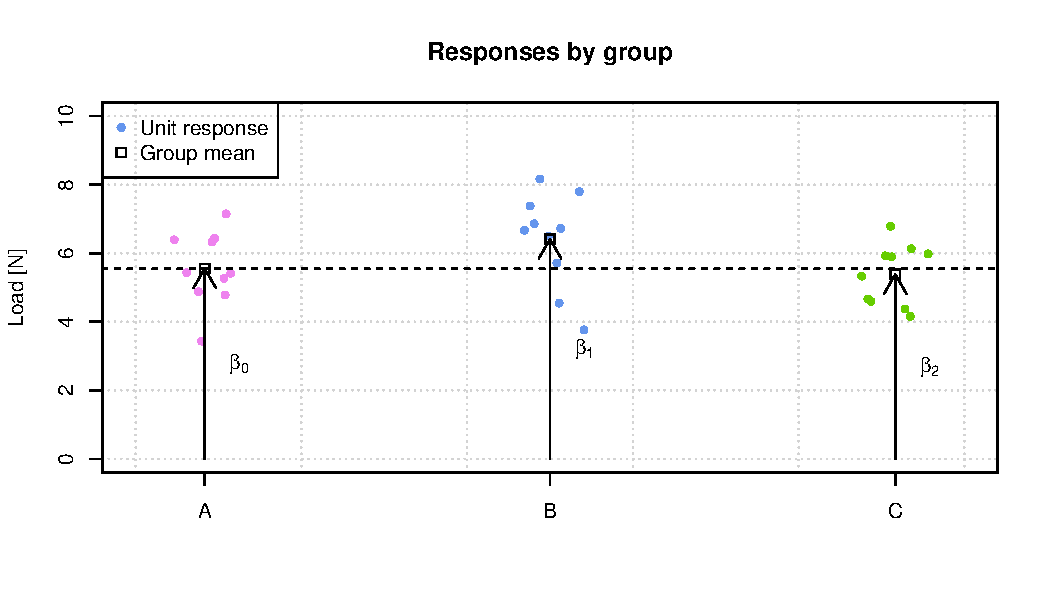
\includegraphics[width=\textwidth]{categorical_regression.pdf}
\caption{Unit responses by group.}
\label{fig:categorical_regression}
\end{figure}

Figure \ref{fig:alt_categorical_regression} shows how the meaning of the regression coefficients could change with choice of encoding. Whereas in Equation \ref{eq:categorical_regression} the fit coefficients were estimates the group means, the coefficients here correspond to the model:
\begin{equation}
	\hat{y} = \hat{\beta}_0 + \hat{\beta}_1x_B + \hat{\beta}_2x_C
\end{equation}
The practical implication of this is that $x_B$ or $x_C$ are now indicator variables for whether a unit deviates from the mean response $\hat{\beta_0}$.
\begin{equation}
	\text{RSS}(\hat{\beta}) = \quad
					\smashoperator{\sum_{i: x_i \in \{x: x_a = 1\}}}(y_i - \hat{\beta}_0) \quad + \quad
					 \smashoperator{\sum_{i: x_i \in \{x: x_b = 1\}}}(y_i - (\hat{\beta}_0 + \hat{\beta}_1)) \quad + \quad
					 \smashoperator{\sum_{i: x_i \in \{x: x_c = 1\}}}(y_i - (\hat{\beta}_0 + \hat{\beta}_2))
\end{equation}
To minimize the first term, $\hat{\beta_0}$ can be set to group A's mean - the other two terms can be minimized by letting $\hat{\beta_1}$ and $\hat{\beta_2}$ correspond to the mean deviation of groups B and C from A.

 Something to be quite careful of is redundantly encoding the groups. If a constant term $\hat{\beta}_4$ were to be included in the model above, then there would be many equivalent ways to express the group effects: $\hat{\beta}_4$ could be any constant value, and $\hat{\beta}_1, \hat{\beta}_2, \hat{\beta}_3$ would be set to deviate from this constant to the group averages. This means that attempts to evaluate Equation \ref{eq:normal_eqtn} will be unsuccessful or unstable\footnote{The instability is caused by numerical errors in calculating the inverse directly.}.
 
\begin{figure}[h]
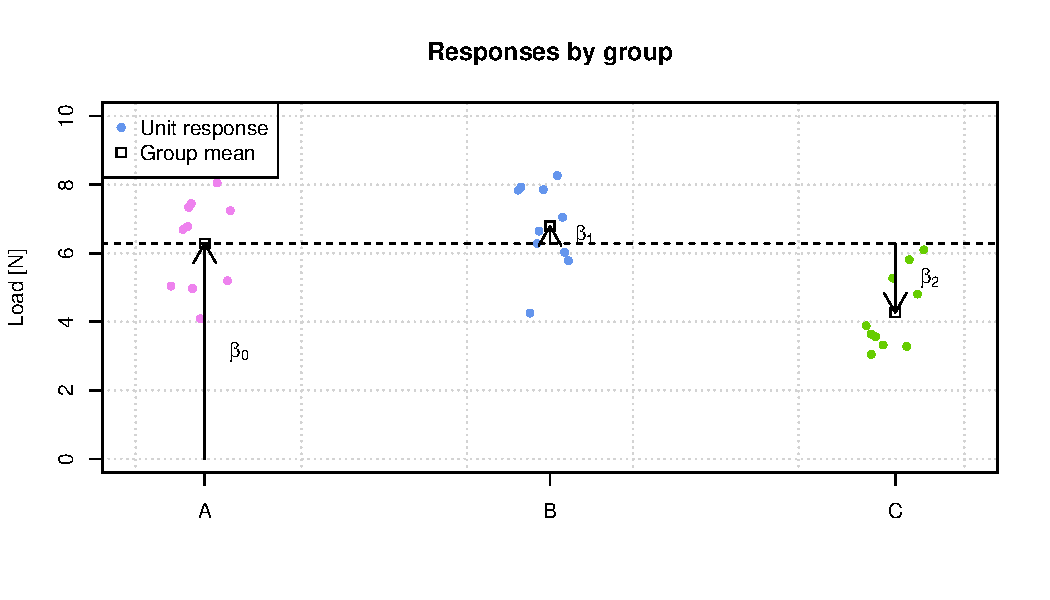
\includegraphics[width=\textwidth]{alt_categorical_regression.pdf}
\caption{Regression coefficients for alteranative categorical encoding.}
\label{fig:categorical_regression}
\end{figure}

The fit of a linear model attempts to estimate the true relationship between the inputs and response. In other words, $\hat{\beta}$ are estimates of the parameters $\beta$:
\begin{equation}
	y = X\beta + \varepsilon
\end{equation}
Where $\varepsilon$ is the error in the response - variation caused by unmonitored variables. In the example, $\beta_1, \beta_2, \beta_3$ are the true group means, and $\hat{\beta}_1, \hat{\beta}_2, \hat{\beta}_3$ are estimates of them. These estimates aren't going to be perfect, and their standard errors can be calculated to get a feel for how accurate they really are. To reemphasize, a standard error is the average difference between an estimate of a parameter over many samples, and the true parameter value. Standard error can be made smaller by reducing the group variance, or by making the sample sizes bigger.  DCA's engineers should seek to minimize variation that isn't relevant to the investigation because this will make it easier to see the effects of the inputs on the reponse for a given sample size. Calculation of standard errors is described and explained in the Appendix.

A reasonable criticism of the above example is that it effectively just a drawn-out calculation of the group sample means. This is true, until the experiment is extended to involve another variable, this time a continuous one, say the volume of a lubricant applied to each design variant. Then the model can be adjustedl to estimate the effects of the lubricant on the load output of each mechanism:
\begin{equation}
	\hat{y} = \hat{\beta}_0 x_A + \hat{\beta}_{1}x_B + \hat{\beta}_{2}x_C + \hat{\beta}_3 x_A x_l + \hat{\beta}_4 x_B x_l + \hat{\beta}_5 x_C x_l
\end{equation}
Where $x_l$ is the volume of lubricant applied, and $\hat{\beta}_3, \hat{\beta}_4, \hat{\beta}_5$ are the change in output force for each design variant per unit volume of lubricant. This model would allow an engineer to see not only how good design variants are relative to one another, but also how much lubricant would need to be applied to bring the performance of one in line with another. Point being, linear models are powerful because they can be adapted to many situations, and because they provide a consistent way of disentangling the effects of experimental treatments.

As an aside, assessing the significance of differences between groups is frequently called Analysis of Variance (ANOVA). It's called this because the analysis focuses on decomposing variation into its sources. Two test statistics, the $t$ and $F$ statistics, can be used to run hypothesis tests on possible sources of variation. Under certain assumptions, these tests provide guidance as to whether a treatment induces an effect or not. It's relevant here because ANOVA can be viewed as linear regression with an emphasis on hypothesis testing. As discussed in the next section, hypothesis tests can be misleading. Furthermore, in complicated models, the canned formulae provided by some statistics resources, certain websites in particular, can become unwieldy and confusing, which could make its results suspect and difficult to explain. By contrast, the structure and basic principles of a linear model are consistent across a variety of model sizes. For this reason, it's suggested that DCA focus on learning to use linear models rather than attempt to use ANOVA.

Linear models would be useful to DCA because they can be used to figure out where variation in a response is coming from, which is the fundamental objective of most experiments. Identifying the factors that have the largest effect on performance, and quantifying those effects, is the first step in understanding how to change a design to make it both better-performing and more robust. Used in combination with multiple-factor experiment designs, linear models could reduce the time and resources taken to conclude an experimental investigation, and would offer a tool for aligning theoretical understanding with empirical evidence.

\newpage
\subsection*{Bayesian Inference}
% What is Bayesian inference?
% How can it be useful to DCA?
% What does it consist of?
% How does it relate to other statistical methods, what are its limitations, and how can it be used for more difficult problems?
Summary statistics such as the coefficients of a linear model or a sample variance state what the most likely value for a parameter\footnote{Reminder: a parameter is a number that controls the shape of a distribution.} is, based on the data alone. They don't say how much more likely this value is is than other values, or let knowledge besides the data be included. In reality, a sample will suggest a distribution of plausible values, and there will be expert knowledge that can be used since it will be known roughly what values are realistic.. Bayesian inference combines readily available knowledge with the experimental data to estimate a distribution of possible parameter values. Figure \ref{fig:annotated_posterior} points out the benefits of making distributional rather than point estimates.
\begin{figure}[b]
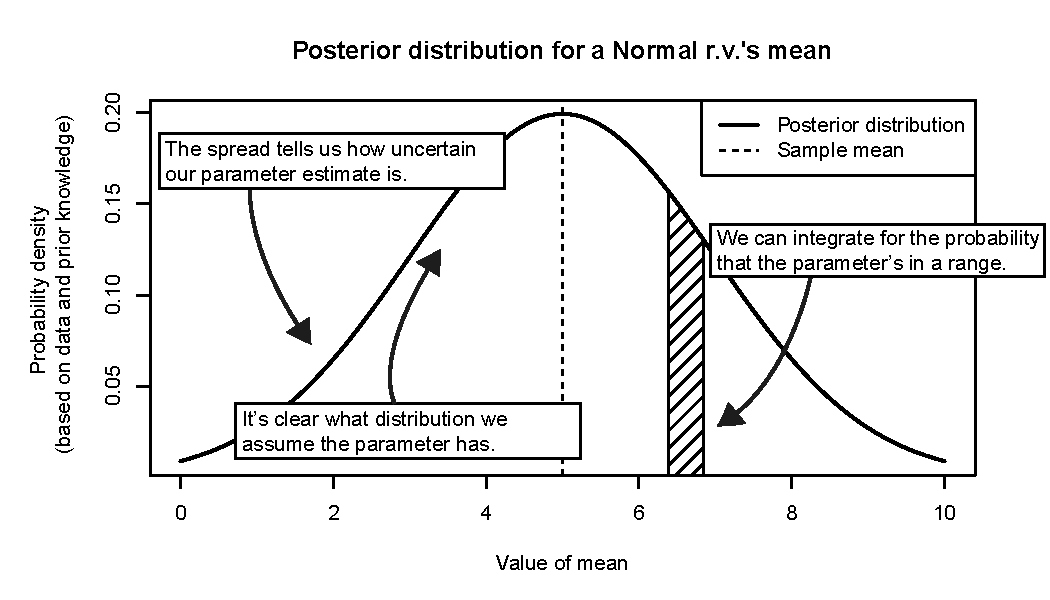
\includegraphics[width=\textwidth]{annotated_posterior.pdf}
\caption{An annotated posterior distribution.}
\label{fig:annotated_posterior}
\end{figure}
\par
Bayesian methods would be useful to DCA because they're more easily understood, visualized, and explained than classical methods\footnote{``Classical methods'' here refers to tools such as hypothesis tests and interval estimates.}, and are relevant to a broader range of situations. They also allow expert knowledge to be used, making it possible to reach a sanitary comprimise between gut-feel and experimental observation. Finally, their emphasis on distribution rather than point estimates better reflects the underlying uncertainty in analytical results. These claims will  be explained in the context of an example.
\par
The proportion of units passing a test is a useful measure of a design's suitability for the problem at hand. Using the results from a test sample and the expertise of an engineering team, and Bayes' theorem, it's possible to estimate what pass rates would be likely if the design were to be produced in larger volumes.
\par
Say that a sample of $n$ units are tested, and $y$ pass. The engineering team collude to sketch out a distribution for the passing rate $\theta$ that's tall near values they think probable and low near ones that seem unlikely. The team is to calculate the probability of a unit passing, given their experimental data and preliminary distribution: Bayes' theorem can be used to do this.
\begin{equation}
  p(\theta|y) = \frac{p(y|\theta)\cdot p(\theta)}{\int_{\theta}p(y|\theta)\cdot p(\theta)\cdot d\theta}
  \label{eq:bayes}
\end{equation}
In words, this means that a passing proportion is more probable if it makes the the number of units that really did pass in the sample more likely and seems sensible to the engineering team. The denominator of this expression is constant w.r.t. $\theta$, making it possible to express the above as:
\begin{align}
  p(\theta|y) &\propto p(y | \theta)\cdot p(\theta)   \label{eq:unnorm_bay} \\
  \small{\texttt{Posterior}} &\propto\small{{\texttt{Likelihood} \cdot \texttt{Prior}}} \nonumber
\end{align}
(\ref{eq:unnorm_bay}) makes it clear that to estimate $p(\theta|y)$, two things are used:
\begin{itemize}
\item The probability of the data - y in n units passing - given a particular population passing proportion, $p(y|\theta)$ (the \emph{likelihood}).
\item  The probability of a passing proportion according to the engineerig team, $p(\theta)$ (the \emph{prior}).
\end{itemize}
In this case, the likelihood is the probability of $y$ units passing and $(n-y)$ units failing. Assuming that passes and failures and independent and that the units come from the same population, then the probability of $y$ passes given that $\theta$ of that population would pass is:
\begin{gather}
  p(y|\theta) = \binom{n}{y} \theta^y (1 - \theta)^{n - y}
  \label{eq:binom_likelihood}
\end{gather}
In a more general sense, the likelihood is the probability of observing the data given that it was being generated according to the model parameterized by $\theta$.
The prior distribution, $p(\theta)$, encodes knowledge of what passing proportions are probable. If the engineering team is unsure what the passing proportion would be, then they may assume that all values are equally likely:
\begin{equation}
  p(\theta) = 1 \qquad \theta \in [0, 1]
  \label{eq:unif_prior}
\end{equation}
Figure \ref{fig:binom_bayes_inference} displays these prior and likelihood distributions. At this point the engineering team can do one of two things: they can evaluate the posterior analytically, or approximate it using a computer. Irrespective of the method chosen, the expression being evaluated is:
\begin{equation}
	p(\theta|y) = \texttt{constant}\cdot p(y|\theta) \cdot p(\theta)
	\label{eq:example_bayes}
\end{equation}
In practice, (\ref{eq:example_bayes}) is calculated using a computer. A grid of $\theta$ values is defined, and their prior probabilities and likelihoods are calculated in line with the functions in (\ref{eq:unif_prior}) and (\ref{eq:binom_likelihood}). This process can be described by the pseudocode:
\begin{align*}
  \quad n &:= \small{\texttt{No. of units tested}} \\
   \quad y &:= \small{\texttt{No. of units that passed}} \\
  \boldsymbol{\theta} & := (0, \ 0.01, \ \dots, \ 1) \\
  \small{\texttt{Prior}} &:= \small{\texttt{Uniform}}(\boldsymbol{\theta}, [0, 1]) \\
  \small{\texttt{Likelihood}} &:= \small{\texttt{Binomial}}(y, n, \boldsymbol{\theta}) \\ 
  \small{\texttt{Posterior}} &:= \small{\texttt{Prior} \odot \texttt{Likelihood}}
\end{align*}
Where $\texttt{Uniform}$ returns the probability density of the uniform distribution for each value in $\boldsymbol{\theta}$ (i.e. a list of ones), $\texttt{Binomial}$ returns the probability of $y$ in $n$ units passing given each of the passing probabilities in $\boldsymbol{\theta}$, and $\odot$ is the element-wise product.
The posterior list would contain the probability density for each passing proportion $\theta$, and is again shown in Figure \ref{fig:binom_bayes_inference}. The pointy part indicates more probable values - a taller, pointier peak represents a more certain estimate because a few values have a much higher probability than lots of others. In the same spirit, the flat prior that was used can be understood as highly uncertain.
\begin{figure}
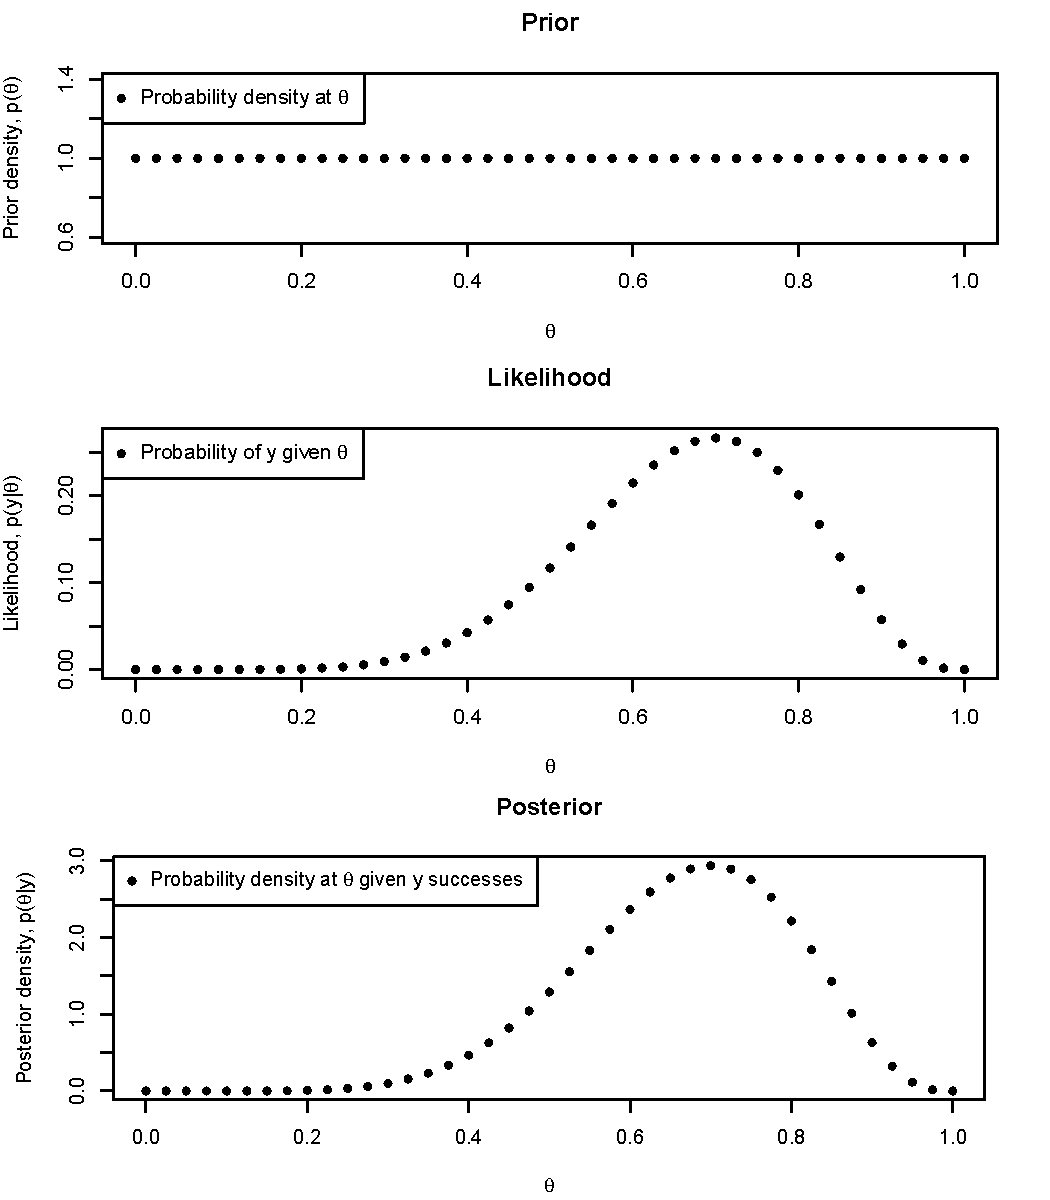
\includegraphics[width=\textwidth]{Bayesian_inference.pdf}
\caption{Combining an uninformative prior with a likelihood distribution to form a posterior distribution of plausible parameter values.}
\label{fig:binom_bayes_inference}
\end{figure}

To recap what's been do so far, the prior knowledge of the engineering team was combined with experimental observations to come up with a likely range of values for the true passing proportion for a population. Taking the product of the prior probability of parameter values with the likelihood of the data produced a posterior distribution indicating the probability of values based on both osurces of information.

Once the posterior has been calculated, it can be used to predict the behaviour of future units. $\tilde{y}$ denotes the number of future units that pass, $\tilde{n}$ is the number of units tested. The probability of $\tilde{y}$ successes, based on the observed data and additional information, is the weighted average of $\tilde{y}$ successes over all possible values of $\theta$:
\begin{equation}
	p(\tilde{y}|y) = \int_{\theta}p(\tilde{y}|\theta, y)\cdot p(\theta|y) \cdot d\theta
\end{equation}
Once again, we can avoid some potentially mischievous mathematics by approximating this integral using a computer: draw samples of $\theta$ based on $p(\theta|y)$, then sample a value of $\tilde{y}$ from $p(\tilde{y}|\theta, y)$. Do this many times and the relative frequency of $\tilde{y}$ values will tend towards $p(\tilde{y}|y)$.
\begin{align}
\small{\texttt{for (i in [1, 10 000]) \{}} &\\
	\tilde{n} &:= \small{\texttt{No. future units to be tested}} \\
	\boldsymbol{\tilde{y}} &:= (0, 1, \dots, \tilde{n}) \\
	\theta &:= \small{\texttt{Sample(}}\boldsymbol{\theta}\small{\texttt{, Posterior)}} \\
	\small{\texttt{Posterior predictive[i]}} &:= \small{\texttt{Sample(}}\boldsymbol{\tilde{y}}\small{\texttt{, Binomial(}}\tilde{y}, \tilde{n}, \theta\small{\texttt{))}}\\
	&\quad\quad \small{\texttt{ \} }}
\end{align}
Figure \ref{fig:posterior_predictive} shows a plot of the posterior predictive, along with the $5\%$ lower limit on the number of units that will pass. This limit can be interpreted as a bound on the plausible number of units to pass, according to the evidence,
\begin{figure}
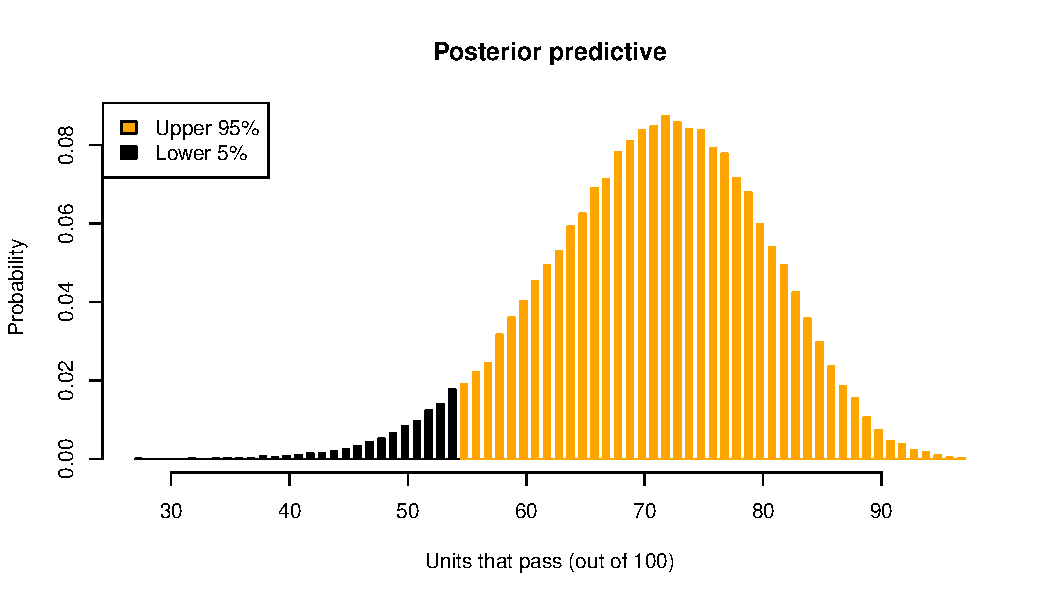
\includegraphics[width=\textwidth]{posterior_predictive.pdf}
\caption{Posterior predictive distribution for the number of passing units in a 100-unit run.}
\label{fig:posterior_predictive}
\end{figure}

The process of inference just described would be valuable to DCA because it would provide a direct representation of how likely particular values are for key performance parameters. Unlike with standard errors, the uncertainty in the estimate is immediately apparent, and the effect of increasing sample size on accuracy is also clear, since the posterior of one analysis can be used as the prior of the next: this means that the information from tests is able to accumulate. This principle is shown in Figure \ref{fig:updating_posterior}, where the flat prior represents initial ignorance about whether a unit will pass: as more units are run, an increasingly narrow peak forms around the most probable passing probability.
\begin{figure}
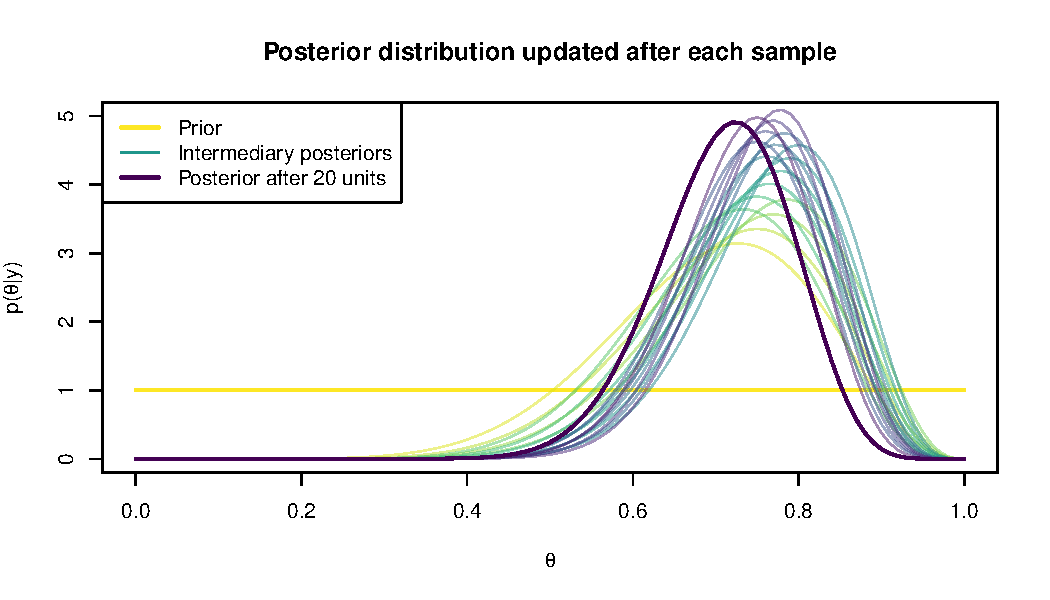
\includegraphics[width=\textwidth]{updating_posterior.pdf}
\label{fig:updating_posterior}
\caption{The uncertainty in the posterior decreases as more samples are conditioned upon.}
\end{figure}
\par

Another advantage of Bayesian methods over hypothesis testing is that it's relatively easy to build models that estimate many parameters simultaneously. An instance of this might be when estimating the mean and the variance of data that's assumed to have a normal distribution. The only change relative to the single-parameter scenario is that we need to define the prior and likelihood in Equation \ref{eq:unnorm_bay} over two parameters instead of one:
\begin{equation}
	p(\theta_1, \theta_2 | y) \propto p(y|\theta_1, \theta_2) \cdot p(\theta_1, \theta_2)
\end{equation}
Where $\theta_1$ is the data's mean, $\theta_2$ is its standard deviation, and $y$ is the dataset. Using a joint prior that weakly favours a range of mean and variance values (based on sensible physical estimates) and a normal likelihood $p(y|\theta_1, \theta_2) = \text{N}(\theta_1, \ \theta_2^{\ 2})$ results in a distribution of parameter values like that shown in Figure \ref{fig:multiparameter_bayes}. This distribution shows how the data reduced uncertainty about what values are reasonable for the mean and standard deviation. This distribution would probably be easier to explain to clients and colleagues than confidence intervals or hypothesis tests.

\begin{figure}
\centering
\makebox[0pt]{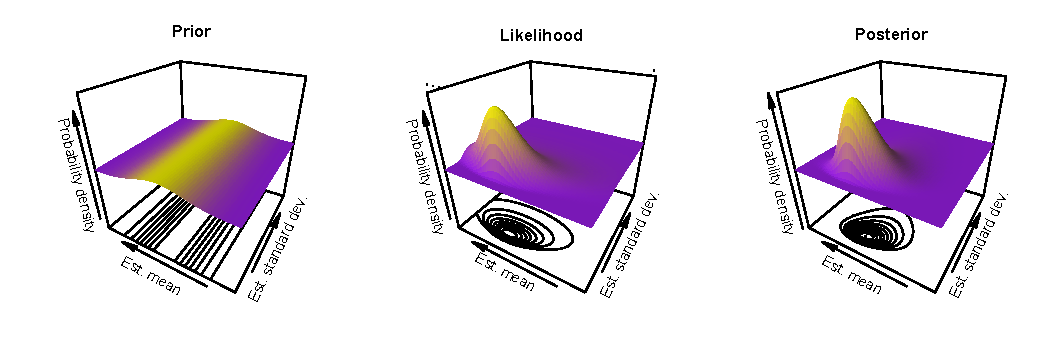
\includegraphics[width=1.4\textwidth]{multiparameter_bayes.pdf}}
\caption{Multiparameter Bayesian inference.}
\label{fig:multiparameter_bayes}
\end{figure}

Shifting from classical methods to Bayesian ones would make statistics within DCA more transparent to both its engineers and clients. Hypothesis tests and interval estimates are easily misinterpreted and are opaque representations of the certainty in parameter estimates, since they are usually presented simply as numerical values. The jargon of classical statistics can make it unclear what's relevant to the problem at hand, and makes an honest explanation of its methods to non-technical team members difficult. Bayesian methods make it clear how the data and prior knowledge are being combined, and provide results that are more easily interpreted. On the other hand, sophisticated Bayesian models require careful thought to be applied effectively, and  may take longer to set up as a result. However, a couple of models could probably answer most questions asked in experimental work, such that once a model is set up it can be used to analyze data from many different experiments.
\par
It is generally recognized that the scientific community as a whole needs to reconsider the practical relevance of hypothesis testing: DCA can hardly be faulted for neglecting to apply ineffective methods. Tolerance and confidence intervals are useful, but can be prone to misinterpretation. 

\subsection*{Markov Chain Monte Carlo}
As mentioned, DCA have previously used Monte Carlo simulation to approximate the distribution of a tolerance chain's dimension. For problems with many parameters - such as a subassembly of many components - Monte Carlo simulation isn't feasible because it would require too many values to be stored in a computer's memory. Instead, the posterior can be approximated using a Markov chain Monte Carlo method, which provides a method for estimating the posterior even if the domain of parameter combinations is extremely large. The details won't be presented here, but in future if DCA should choose to construct models containing many parameters they will probably need to use it. The basic idea is to generate a sequence of values according to their relative probabilities, such that the relative frequency of values in the chain converges towards the posterior distribution. 

%%
\section{Presentation \& Visualization}
\subsection{Why Visualization is Important}
Good visualization exposes patterns in data in a way that's immediately interpretable and precise. A visualization is a mapping from the numerical domain of a dataset to the visual domain of a plot. Data isn't stored in a way that can be interpreted easily, so it needs to be transformed for it to be useful - maths is one means of transforming it to reveal patterns, and plots are another.

DCA's use of visualization could be improved by:
\begin{itemize}
\item Presenting summary plots rather than raw data where appropriate.
\item Providing only as much information as is needed to understand the results - is the entire group's results necessary, or just one unit's?
\item Using plots to understand data as well as present it - in the same way that fiddling with prototypes inspires ideas, visual representations of data can suggest things that aren't clear in formal analyses.
\item Faceting line plots - overlaid line charts are crude representations of data that will generally only show obvious differences. This is mentioned because of DCA's reliance on line plots.
\end{itemize}
Designing a visualization means giving thought to:
\begin{itemize}
\item Data - are the variables continuous, categorical, or ordered categorical?
\item Geometry of datapoints - points, lines, or bars
\item Datapoint aesthetics - color, size, shape, and position of the geometries
\item Scales - mappings from data to aesthetics
\item Summary statistics - plottable summaries of the data
\item Facets - plotting subsets of the data separately
\item Themes - typeface, non-data colours, axes and so on.
\end{itemize}
This many elements may seem overwhelming, and can be justified, although the most important ones are choice of geometry, aesthetics, and scales. Aesthetics can represent dimensions that aren't displayed via a plot's axes. Geometry carries information such as resolution, chronology,  and connectivity. Scales can skew perception of effects, and should be chosen carefully.

 In DCA, experimental results are regularly discussed in team meetings. These discussions are guided by charts of the results; the conclusions of these meetings will guide an experimental investigation, and can only be as well-informed as those charts permit. If charts contain irrelevant or misleading information, an investigation may stall.
  While default options in programs like Excel and Matlab can be very useful for quickly surveying data, they are rarely ideal for focusing technical discussions. The same applies to plotting raw time series data directly - gross structure can be made apparent, but there will almost certainly be both a clearer way to express it and relevant information will be submerged in a sea of noise.

To show what's meant by the above criticism, consider Figure \ref{fig:}, which is an imitation of the plot shown in Figure \ref{fig:line_chart}. 

\begin{figure}
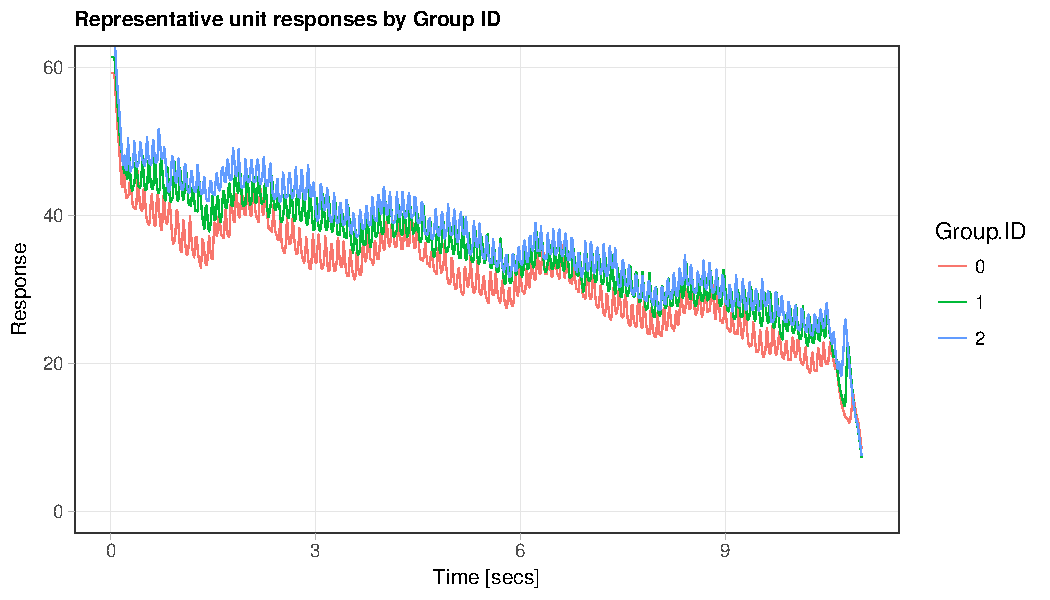
\includegraphics[width=\textwidth]{thinned_line_chart.pdf}
\end{figure}

\begin{figure}
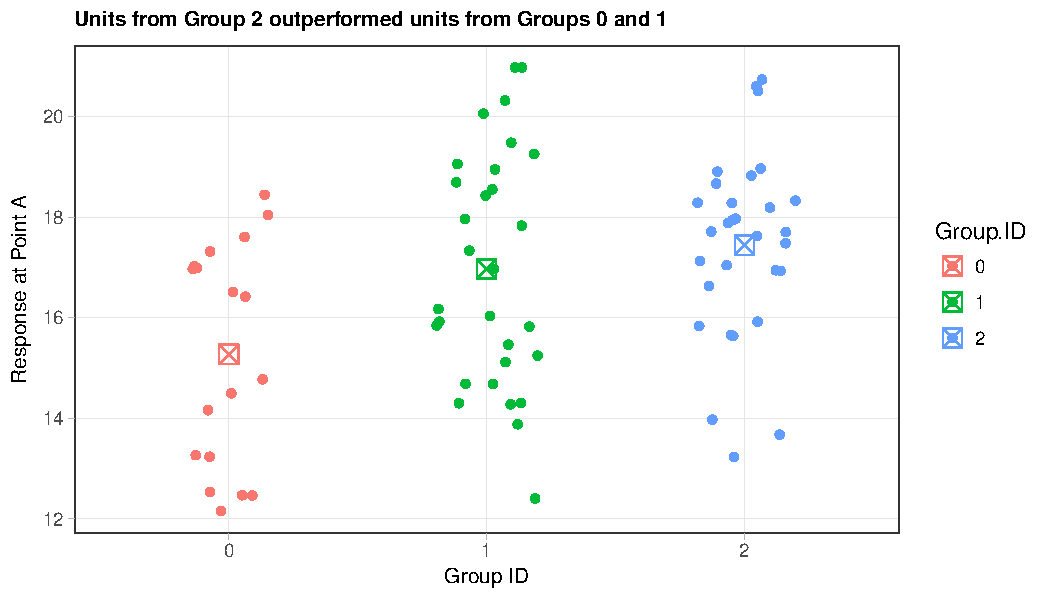
\includegraphics[width=\textwidth]{strip_plot.pdf}
\end{figure}

\begin{figure}
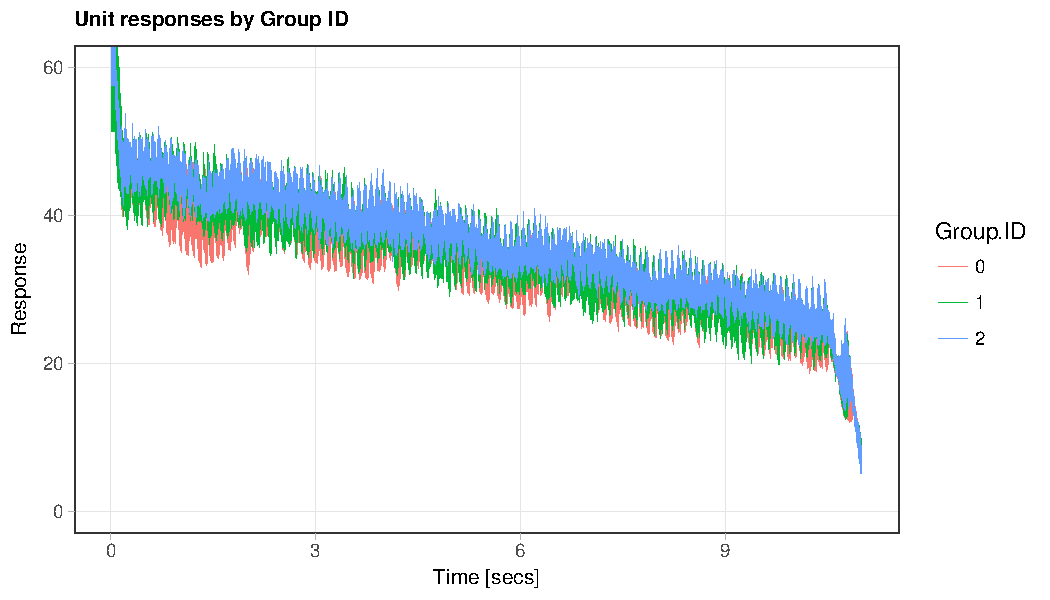
\includegraphics[width=\textwidth]{imitation_line_chart.pdf}
\end{figure}

\begin{figure}
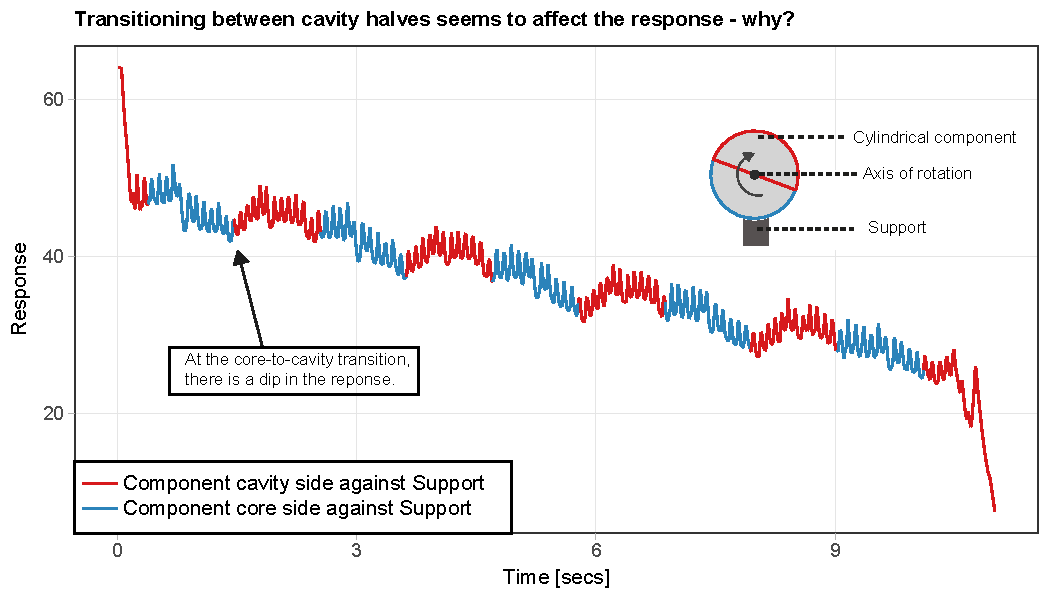
\includegraphics[width=\textwidth]{annotated_line_chart.pdf}
\end{figure}

\cite{hastie2013elements}, \cite{gelman2013bayesian}, \cite{faraway2004linear}, \cite{blitzstein2014linear}, \cite{jaynes2003probability}, \cite{wickham2009ggplot2}, \cite{montgomery2000design}, \cite{kruschke2015doing}, \cite{iso2014statistical}.


%%
\section{Software}
\begin{itemize}
\item Excel
\item Matlab
\item R
\item Python
\item Minitab
\end{itemize}

\newpage


%% CONCLUSIONS AND RECOMMENDATIONS %%
\chapter{Conclusions \& Recommendations}


\newpage
%% BIBLIOGRAPHY
\bibliographystyle{ieeetr}
\bibliography{icr}

\newpage
%% APPENDIX %%
\appendix
\chapter{}
\subsection{What is probability theory, and what is a probability?}
Probability allows us to analyze a system without requiring complete mechanical knowledge of it. `'Randomness'' refers to sources of variation that aren't measured. You may have heard of probabilities as representing `'Degrees of belief''. To understand what a belief is, consider this example. We machine a coin that we check is a symmetric disk of homogeneous density. I flip the coin ten times, and it comes up heads every single time. You might be surprised by this, and accuse me of flipping it in a controlled way. I then ask you how I can flip it in a way that is fair. What is your response?
\par
If you say that it should come heads as many times as tails, then the experiment is no longer random, as we know what the outcome will be. You may gesticulate and say ``You need to flip it \emph{randomly}''. I would press you to tell me what this means - I require a mechanism to decide how to flip the coin, and physical mechanisms are deterministic.
\par
Point being, the probability of an outcome can only be evaluated relative to a set of assumptions you make about the mechanism generating those outcomes. You had a preconceived notion that the way I flipped the coin would favor neither heads nor tails, and therefore saw ten heads as supremely improbable. It is exactly these kinds of assumptions that form the basis of statistical analyses. Being able to express physical assumptions mathematically gives an analytical voice to our physical understanding of the world, and should ideally feel as natural as that understanding.
\newpage

\subsection{Standard Error of a Sample Mean}
We can see this by recognizing that the sum of independent observation's variances is equal to the variance of the sum of the observations:
\begin{align}
 \text{Var}\sum_{i = 1}^n X_i &= \sum_{i = 1}^n \text{Var}X_i\\
	\text{Var}n\bar{X} &= n\text{Var}X \\
	\implies \sqrt{\text{Var}\bar{X}} &= \frac{\sigma}{\sqrt{n}}
\end{align}
\par
Analytically, we can solve for $p(\theta|y)$ directly
\[
  p(\theta|y) \propto \binom{n}{y}\theta^y (1 - \theta)^{n-y}\cdot 1
\]
To find the constant of proportionality, we need to divide the r.h.s. by its integral over all values of $\theta$, such that the $\int_0^1 p(\theta|y)\cdot d\theta = 1$. As it happens, the r.h.s. has the form of what's called a beta distribution
\[
  p(x; a, b) \propto x^{a - 1}\cdot x^{b-1}
\]

\subsection{Confidence intervals}
\[
	 = \text{P}\Bigg(\frac{\Big(\frac{\bar{x} - \mu}{\sigma/\sqrt{n}}\Big)}{s/\sqrt{n}\sigma}\Bigg)
\]


\subsection{Justifications for Least-Squares Regression}
\begin{gather}
	\text{Assume that the errors in $y$ given $x$ are normal with constant variance and mean zero}\\
	\epsilon \sim \text{N}(0, \sigma^2) \\
	p(\epsilon|\hat{\beta}) = \frac{1}{\sqrt{2\pi}\sigma} \exp (-\frac{\epsilon^2}{2\sigma^2})
\end{gather}
Assume that the true response is a linear function in $\hat{\beta}$, such that $E(Y|X) = X\hat{\beta}$, then take the log of the likelihood:
\begin{gather}
	l(\hat{\beta}) \propto -(Y - X\hat{\beta})^2
\end{gather}
Such that maximizing the likelihood is equivalent to minimizing the RSS criterion.

The final way to justify a least squares fit does not require a normality assumption: instead, it is rationalized as providing the lowest variance estimate of $EY$ for a given $X$. In other words, a least squares fit will, on average, be closer to the true response than a linear fit made in some other way.

Start by assuming that $y$ truly is a linear function of $X$, which is a vector of inputs, so that:
\begin{gather}
	E[y|X] = X\hat{\beta} 
\end{gather}
Next note that it follows from the above that the least squares fit will be an unbiased estimate, provided that $\boldsymbol{y}$ is drawn i.i.d. at a given $X$:
\begin{gather}
	E[X\hat{\hat{\beta}}] = E[\boldsymbol{X(X^T X)^{-1}X^T y}] \\
	= \boldsymbol{X(X^T X)^{-1}X^T X}\hat{\beta} \\
	\implies E[X\hat{\hat{\beta}}] = \boldsymbol{X}\hat{\beta}
\end{gather}
Almost there. Now we need to think about other possible estimates of $E[y|X]$. We can see from (16) that our estimate is a linear function of $y$ (Estimable functions?). Imagine another function $\boldsymbol{c^T y}$ that's also linear in $\boldsymbol{y}$. The Gauss-Markov theorem states that the variance of the least-squared estimate is guaranteed to be less than this other linear estimate:
\begin{equation}
	\text{Var}(\boldsymbol{X}\hat{\hat{\beta}}) \leq \text{Var}(\boldsymbol{c^Ty})
\end{equation} 
The proof for this is:
\begin{gather}
	E[(a^T \hat{\hat{\beta}} - a^T \hat{\beta})^2] \leq E[((c^T y - a^T \hat{\hat{\beta}}) - ( a^T \hat{\beta} - a^T \hat{\hat{\beta}}))^2]\\
	\leq  E[((c^T y - a^T \hat{\hat{\beta}}) + ( a^T \hat{\hat{\beta}} - a^T \hat{\beta}))^2] \\
	\leq E[(c^T y - a^T \hat{\hat{\beta}})^2] + E[( a^T \hat{\beta} - a^T \hat{\hat{\beta}})^2] \\
	\iff 0 \leq E[(c^T y - a^T \hat{\hat{\beta}})^2]
\end{gather}
Is this is a proof? How can you be sure?


\end{document}